\documentclass[12pt,a4paper]{article}
\usepackage[utf8]{inputenc}
\usepackage[brazil]{babel}

% Permite colocar figuras lado a lado ou
% fazer posicionamentos arbitrários
\usepackage[lofdepth,lotdepth]{subfig}
\usepackage{graphicx}
% Diretório padrão para figuras
\graphicspath{ {images/} }

\usepackage{hyperref}
\usepackage{abnt-alf}
\usepackage[top=3cm,bottom=2cm,left=3cm,right=2cm]{geometry}
\usepackage{indentfirst}
\usepackage{csquotes}

% Prefine que parágrafos (\paragraph) sejam colocados
% no índice. Isse permite usá-los livremente para
% formatação, caso contrário temos um erro se eles não
% estiverem dentro de uma subsubsection.
\setcounter{tocdepth}{3}

% Adiciona o comando \source para citar fontes abaixo
% de figuras. Muito útil!
\usepackage{caption}
\newcommand{\source}[1]{\vspace{-10pt} \caption*{Fonte: {#1}} }

% Facilita o copy 'n paste no PDF
% Remove ligaturas na cópia
%\input{glyphtounicode}
%\pdfgentounicode=1

% Texto colorido e afins. Bom para TODO notes
\usepackage{xargs}
\usepackage[pdftex,dvipsnames,table,xcdraw]{xcolor}
\usepackage[normalem]{ulem}
\useunder{\uline}{\ul}{}

% Símbolos diferentes para o texto, como setas →,
% símbolos de copyright e trademark, euro, etc.
% Não é muito útil, mas de vez em quando ajuda.
% Ao invés do comando do latex, dá pra usar o
% caractere em UTF-8.
\usepackage{textcomp}

% Todo notes.
% Muito útil para deixar anotações enquanto se está
% construindo o texto, depois dá para remover e onde
% quebrar são comentário que devem ser removidos.
\usepackage[colorinlistoftodos,prependcaption,textsize=tiny]{todonotes}
\newcommandx{\question}[2][1=]{\todo[linecolor=red,backgroundcolor=red!25,bordercolor=red,#1]{#2}}

\newcommandx{\change}[2][1=]{\todo[linecolor=blue,backgroundcolor=blue!25,bordercolor=blue,#1]{#2}}

\newcommandx{\info}[2][1=]{\todo[linecolor=OliveGreen,backgroundcolor=OliveGreen!25,bordercolor=OliveGreen,#1]{#2}}

\newcommandx{\draft}[2][1=]{\todo[linecolor=Plum,backgroundcolor=Plum!25,bordercolor=Plum,#1]{#2}}

\newcommandx{\thiswillnotshow}[2][1=]{\todo[disable,#1]{#2}}
\reversemarginpar
% END Todo notes.

\begin{document}

% CAPA
\pagestyle{empty}
\begin{center}
\large  \textbf{UNIVERSIDADE PRESBITERIANA MACKENZIE}
\large  \textbf{PROGRAMA DE PÓS-GRADUAÇÃO EM}\\
\large  \textbf{ENGENHARIA ELÉTRICA E COMPUTAÇÃO}\\
\vskip 2.0cm
\textbf{\large Ronie Miguel Uliana}\\
\vskip 4.0cm
\setlength{\baselineskip}{1.5\baselineskip}
\textbf{\MakeUppercase{\large Título a ser Definido}}\\
\vskip 4.5cm
\end{center}
\hfill{\vbox{\hsize=8.5cm\noindent\strut
Projeto de Pesquisa apresentado ao Programa\break
de Pós-Graduação em Engenharia Elétrica e\break
Computação da Universidade Presbiteriana\break
Mackenzie como parte dos requisitos para a\break
aprovação na disciplina de Metodologia do\break
Trabalho Científico.}\\
\strut}
\vskip 3.0cm
\textbf{\normalsize Orientador: Prof. Dr. Leandro Nunes de Castro}\\
\vskip 2.0cm
\begin{center}
São Paulo\\
2017\\
\end{center}

% RESUMO
\newpage
\thispagestyle{plain}
\pagenumbering{roman}
\begin{center}
\large
\textbf{RESUMO}
\end{center}
\renewcommand{\baselinestretch}{0.6666666}
A ser definido
\\[0.5cm]
\begin{flushleft}
{\bf Palavras-chave:} {\it apresentação, separada por vírgulas, de três a seis unitermos significativos para o trabalho.}
\end{flushleft}

% SUMÁRIO
\newpage
\thispagestyle{empty}
\tableofcontents

% DESENVOLVIMENTO
\newpage
\pagestyle{plain}
\pagenumbering{arabic}
\renewcommand{\baselinestretch}{1.5}
\normalsize

\listoftodos[Notas]

\section{INTRODUÇÃO}

% Ronie 2017-04-02 Professor, usei seu texto com praticamente nenhuma modificação aqui. Conforme o trabalho anda, vamos refinando, mas gostei do texto.
Ao longo da vida profissional é comum para o indivíduo passar por diversas movimentações de carreira. Um estudante de engenharia pode iniciar como Trainee em uma empresa e progredir para Engenheiro, Supervisor de Obras e Diretor de Engenharia. Na área de computação é possível ver um Programador se tornar Analista-Programador, Coordenador de Desenvolvimento, Gerente de Projetos, chegando até Diretor de Operações. Esses são casos em que a movimentação de carreira segue um padrão mais tradicional de progressão, mas também há situações extremas de transições de carreira na qual um Analista-Programador resolve se tornar um Chef de Cozinha. Em qualquer um dos casos, as movimentações de carreira são sempre uma etapa de grande relevância profissional e que, ao mesmo tempo, podem causar muito estresse, insegurança e alguns desconfortos pelos novos desafios que surgirão.

Partindo do histórico profissional de 10 milhões de pessoas, este projeto de pesquisa usa o Mapa de Carreiras da empresa Vagas Tecnologia~\todo{Ronie 2017-04-02: Verificar se podemos usar o nome da empresa} com o objetivo de fazer um estudo analítico sobre a movimentação de carreira de profissionais da área de tecnologia no Brasil entre os anos 2010 e 2016. O problema é modelado com uma estrutura em grafos e são usados conceitos e ferramentas de Mineração de Dados, Redes Complexas, Teoria de Grafos e Bancos de Dados Não-Relacionais no tratamento analítico dos dados.

\draft[inline]{Abaixo algumas frases incompletas com ideias}

\ldots Esse trabalho se propõe a transformar um banco de dados relacional em um banco de dados de grafo.

\ldots a colocar os dados de milhões de currículos em um arcabouço que permita a exploração de padrões de movimentação de trabalho no mercado brasileiro.

\ldots a explorar um banco de dados de currículos para compreender como o mercado de trabalho brasileiro se quanto a movimentação dos profissionais.

\section{JUSTIFICATIVA}

Existem diversos trabalhos sobre movimentação profissional, principalmente sobre os fatores que motivam a mudança, como os expostos por~\citeonline{Ng2007-zp}~\info{Impact Factor: 2.419 (2012)}\todo{Ronie: tem mais uma série de papers, ler e mencionar (na introdução, talvez?)}. Porém, dos trabalhos que tratam explicitamente de progressão de carreira, poucos são baseados em bancos de dados de grande volume~\cite{Cetintas2011-op,Xu2014-gj,Xu2015-jb} ou focam em profissionais da área de computação~\cite{Qu2016-dy}. No Brasil, não foram encontrados trabalhos dessa natureza, ponto onde essa dissertação traz uma grande contribuição.

% NA JUSTIFICATIVA/MOTIVAÇÃO É INTERESSANTE MENCIONAR QUE A CONTRIBUIÇÃO DA DISSERTAÇÃO NÃO É APENAS TÉCNICA, TRAZ TAMBÉM UMA MAIOR COMPREENSÃO SOBRE AS MOVIMENTAÇÕES DE CARREIRA DA ÁREA DE TI NO BRASIL

Esse trabalho aborda o problema de \textit{progressão de carreira} usando técnicas de Mineração da Dados para gerar conhecimento a partir de uma base de dados de mercado. Os dois aspectos centrais desse trabalho são, portanto, o uso de uma base de dados real e a aplicação de métodos analíticos para a extração de conhecimentos a partir dessa base.

% SUGIRO SUBSTITUIR BANCO DE DADOS POR BASE DE DADOS, POIS A ÚLTIMA INDEPENDE DE TECNOLOGIA

As ocupações que formam a base de dados são preenchidas espontaneamente pelos usuários do sistema. Como não são preenchidas a partir de uma lista pré-selecionada, os títulos que compõem a lista final de ocupações refletem diretamente como as pessoas realmente se referem à própria profissão. % NÃO SERÁ NECESSÁRIO NORMALIZAR ESSE PREENCHIMENTO?

A base de dados possui uma dezena de milhões de pessoas registradas, o que representa uma amostra significativa da população brasileira economicamente ativa. Esse volume permite um alto grau de confiança nos valores obtidos pela análise.

% PARA A BASE DE COMPUTAÇÃO QUE VAMOS TRATAR PRECISAMOS INFORMAR O NRO EXATO DE PESSOAS E PROFISSÕES A SEREM USADOS

\todo[inline]{Ronie: tenho a confiança para salários já calculada, será que dá para calcular a confiança da migração?}

Pelos motivos acima, acredita-se~\todo{Ronie: Achei ruim isso. Ajuda, pls!} que esses resultados possam ser usados como uma das fontes para trabalhos nesse assunto.

Por exemplo, na indústria, ele pode ser usado para consulta de cargos e salários, pode servir de base para elaboração de planos de carreira ou para busca de profissionais alternativos no momento da contratação.

Academicamente, esse trabalho pode ser usado como fonte para pesquisas em áreas sociais que envolvam o mercado de trabalho de computação.

O setor público possui a iniciativa da Classificação Brasileira de Ocupações (CBO). Ela é uma lista classificatória das ocupações no mercado de trabalho e é elaborada pelo Ministério do Trabalho em colaboração com IBGE, sindicatos e empresas privadas. Atualmente ela classifica cerca de 2.500 ocupações em pouco mais de 600 grupos, sua última versão é de 2010~\cite{mte-cbo-tc}. O trabalho presente pode servir como uma das fontes para atualização da CBO, principalmente quanto às novas ocupações.

Finalmente, para profissionais da área ele pode indicar alternativas na progressão de carreira e o que esperar nesse caminho, por exemplo.

\section{REFERENCIAL TEÓRICO}
% NESTE MOMENTO VOU PULAR O REFERENCIAL E VOU PARA A SEÇÃO DE METODOLOGIA

% Ronie 2017-04-02: Deixei a introdução que você escreveu, Professor.
O objetivo deste capítulo é oferecer as bases conceituais necessárias ao estudo analítico das movimentações de carreira na área de tecnologia, como discutido anteriormente. Os principais conceitos necessários à pesquisa são: Mineração de Dados; Redes Complexas; Teoria de Grafos; e Bancos de Dados Não-Relacionais. Cada um deles será apresentado como uma seção do capítulo, enfatizando apenas os aspectos necessários ao estudo analítico do projeto.

Os dados são trabalhados para encontrar padrões sobre evolução de carreira e movimentação no mercado de trabalho. As técnicas específicas de Mineração de Dados são apresentadas também nessa seção. Em especial, são apresentados conceitos básicos sobre agrupamento dos dados em grafos (\textit{Clustering})~\footnote{Ronie 2017-03-22: os PDFs que separei com as carreiras}, estatística não-paramétrica~\footnote{Ronie 2017-03-22: as KDEs geradas para salários} e similaridade entre sequências~\footnote{Ronie 2017-03-22: Pensei aqui na recomendação de próximo cargo, como em \citeonline{Xu2014-gj}}.

Para facilitar a compreensão do texto, abaixo são apresentadas definições para os termos encontrados no restante desse trabalho. Os significados são baseados livremente nos trabalhos de \citeonline{Wickham2014-qh} e \citeonline{Nunes2016}.

\question[inline]{Ronie 2017-04-02: Dúvida... qual seria o melhor formato para essas definições? Seriam subseções? Uma tabela? Texto corrido? Um apêndice? Por enquanto coloquei como "parágrafos", no jargão do Latex.}

\paragraph{Definição 1}
\textit{Dados} são símbolos, textos ou números sem significado atribuído. Por exemplo, 2014, \enquote{verde} ou $\lambda$.

\paragraph{Definição 2}
\textit{Informação} é um dado associado a um significado. Por exemplo, o câmbio entre Real e Dólar ser 3,10 no dia de hoje ou então que a última manutenção da estrada SP-250 foi em 2012.

\paragraph{Definição 3}
\textit{Conhecimento} é uma informação que possui significado associado suficiente para a tomada de decisões. Por exemplo, saber que o dólar vai subir ou saber que as estradas para o interior estão em más condições.

\paragraph{Definição 4}
\textit{Base de Dados} ou \textit{Conjunto de Dados} é o conjunto de dados disponível.

\paragraph{Definição 5}
\textit{Tabelas} são dados organizados em formato tabular onde as linhas são chamadas \textit{registros} ou \textit{objetos} e as colunas são chamadas \textit{atributos} ou \textit{variáveis}. Uma tabela representa um conjunto de registros de um mesmo tipo.

\paragraph{Definição 6}
Um \textit{Objeto}, \textit{Registro} ou \textit{Dado} descreve uma \enquote{unidade} sobre a qual temos informações.

\paragraph{Definição 7}
Um \textit{Atributo}, \textit{Campo} ou \textit{Variável} representa uma característica comum a todos os registros de um mesmo tipo. Um atributo dá significado a um valor.

\paragraph{Definição 8}
Um \textit{Valor} é o conteúdo de um atributo em um registro. Ele pode ser numérico, representando uma medição, grandeza ou ordem; um classe, representando um tipo ou classificação do registro; ou um texto, representando informação não estruturada.

% ==========
\subsection{Descoberta de Conhecimento em Bases de Dados}

\enquote{Knowledge Discovery in Databases is the non-trivial process of identifying valid, novel, potentially useful, and ultimately understandable patterns in data}~\cite{Fayyad1996-yz}.

A Descoberta de Conhecimento em Bases de Dados (Knowledge Discovery in Databases - KDD) é o processo de identificar novos padrões válidos e úteis em dados. Essa é uma área ampla e convenciona-se chamar \textit{Mineração de Dados} a parte de KDD que trabalha o processo de descoberta do conhecimento~\cite{Nunes2016}.

A Mineração da Dados pode ser dividida em três processos principais aplicados a partir de uma ou mais Bases de Dados: a Preparação dos Dados, a Mineração em si e a Validação do Conhecimento~\cite{Nunes2016}.

A Preparação consiste em processos para extrair as informações das bases da dados e torná-las adequadas para o uso nas etapas seguintes do processo. A primeira etapa da preparação lida com a \enquote{limpeza} dos dados, ou seja, a remoção ou tratamento de dados que podem distorcer os resultados das análises estatísticas e algoritmos. As etapas seguintes da preparação tratam da integração dos dados quando esses vêm de fontes diferentes: redução, quando o número de objetos ou campos dificulta a mineração; e a transformação e discretização, capazes de adaptar os dados aos algoritmos de mineração.

A Mineração em si é a parte do processo na qual são aplicados algoritmos capazes de descrever e extrair conhecimentos úteis e não-triviais dos dados. As principais tarefas associadas a essa etapa envolvem a análise descritiva dos dados, análises exploratórias, análises preditivas, identificação de relacionamento entre atributos (associação) e detecção de anomalias. A decisão de quais tarefas serão executadas e quais algoritmos serão aplicados depende principalmente da informação procurada, mas é limitada pelo formato e disponibilidade dos dados.

A Validação do Conhecimento é a etapa em que os conhecimentos descobertos são verificados quanto à validade e utilidade. A participação de especialistas nesse processo é essencial.

\subsubsection{Mineração de Dados}

A Mineração de Dados usa algoritmos para extrair conhecimento das bases de dados já preparadas~\cite{Nunes2016}.

A analogia\ldots

Existem quatro áreas principais que contribuem com técnicas para o que é conhecido hoje como Mineração de Dados: Estatística, Inteligência Artificial, Aprendizado de Máquina e Computação Natural~\cite{Gorunescu2011-oa}.

A Estatística contribuiu diretamente com a Análise Exploratória de Dados e Análise Descritiva~\cite{Gorunescu2011-oa}. Essas são as primeiras etapas na Mineração de Dados e servem para orientar as etapas posteriores, a seção~\ref{sec:analise-exploratoria} detalha melhor ambas.

A Inteligência Artificial contribuiu com técnicas de processamento da informação e racionalização (?reasoning?).

O Aprendizado de Máquina permite criar modelos automáticos usando uma parte dos dados. \citeonline{Gorunescu2011-oa} também considera a Computação Natural como um grande contribuidor nesse mesmo contexto.

[Completar\ldots]

\subsubsection{Análise Exploratória de Dados e Análise Descritiva}\label{sec:analise-exploratoria}

A \textit{Análise Exploratória dos Dados} (Exploratory Data Analysis - EDA) foi inicialmente introduzida por \citeonline{Tukey1977-of} em sua percepção que os estatísticos da época davam importância excessiva a confirmação de hipóteses sem compreender corretamente os dados com os quais trabalhavam~\cite{Fernholz2000-rj}. Tukey acreditava que uma ênfase igual deveria ser dada tanto à formulação da hipótese quanto a sua confirmação.

A EDA promove principalmente o uso de gráficos e de estatística descritiva para compreensão dos dados. Não coincidentemente, essas são as primeiras etapas da Mineração de Dados.

Uma das primeiras tarefas exploratórias consiste em entender, resumidamente, qual a distribuição dos valores dos atributos. Para atributos numéricos, \citeonline{Hoaglin1983-aq} advogavam o uso do \enquote{resumo de cinco números} (five-number summary), ele é um conjunto que resume a distribuição das observações usando cinco estimadores. São eles: a mediana, o primeiro e terceiro quartil, a mínima e a máxima. Esses cinco números são a base do gráfico de \textit{box and whiskers}, disponível na maior parte dos softwares estatísticos. Também é possível derivar outras estimativas a partir desses números, como o intervalo interquartil e a amplitude.

\begin{figure}[ht]
  \centering
  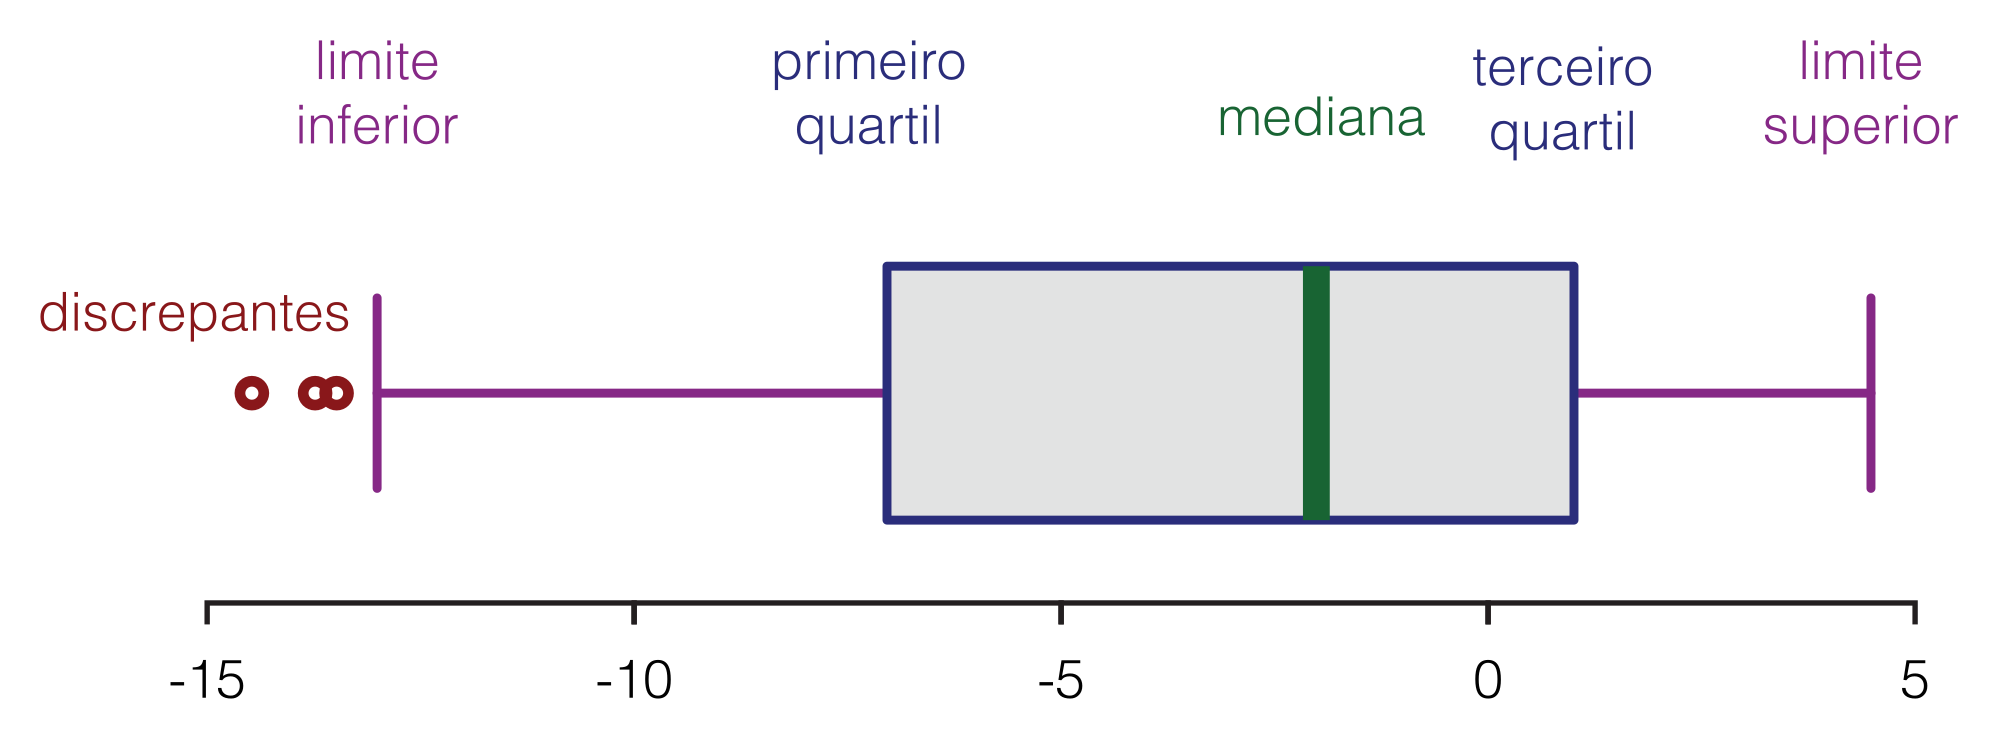
\includegraphics[scale=0.16]{BoxPlot.png}
  \caption{\textit{Box and Whiskers}}
  \label{fig:descricao-box-and-whiskers}
  \source{CEPID NeuroMat}
\end{figure}

Outra variação é o \enquote{resumo de sete números} (seven-number sumary), descrita primeiramente por Bowley (ref). Nela, o resumo é constituído pelos valores extremos, os decis inferior e superior, os quartis inferior e superior e a mediana.

Ambas as abordagens, principalmente quando apresentados em formata gráfico, permitem uma checagem rápida sobre a normalidade da distribuição, sua inclinação e sua variabilidade. Vários estimadores e testes estatísticos assumem distribuições normais e essa checagem permite identificar quais abordagens são mais facilmente trabalháveis.

Pode-se descrever dados categóricos ou ordinais a partir de uma \textit{distribuição de frequências}. Para isso, basta contar o número de ocorrências para cada valor distinto do atributo~\cite{Nunes2016}.

No caso de dados categóricos, um gráfico de barras ordenado de maneira decrescente pelo número de ocorrências cria um \textit{gráfico de Pareto}. Esse gráfico indica rapidamente qual o valor mais frequente, o menos frequente e qual o tamanho da discrepância no seus números de ocorrências. Uma linha com a frequência acumulada completa o gráfico, como observado na figura \ref{fig:exemplo-pareto}.

Em atributos ordinais, que possuem uma ordem natural, o mesmo gráfico com as barras ordenadas pelo próprio atributo o transforma em um \textit{histograma}. O histograma possui características parecidas com o de Pareto e é uma estimativa visual da distribuição das frequências.

\begin{figure}[ht]
  \centering
  \subfloat[][Histograma] {
  	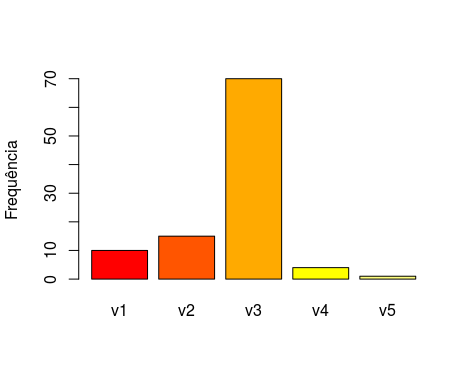
\includegraphics[scale=0.5]{histograma.png}
    \label{fig:exemplo-pareto}
  }
  \subfloat[][Gráfico de Pareto] {
  	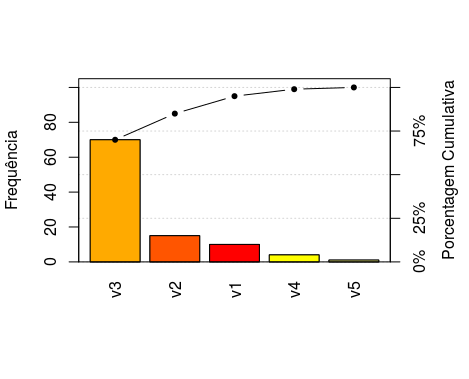
\includegraphics[scale=0.5]{pareto.png}
  }
  \caption{Exemplo de histograma e gráfico de Pareto}
  \label{fig:exemplos-pareto-histograma}
  \source{Elaboração do autor}
\end{figure}

Valores numéricos podem ser transformados em histogramas ou gráficos de Pareto se passarem por uma transformação chamada \textit{discretização}.

A discretização converte dados numéricos em dados categóricos dividindo os valores possíveis do atributo em intervalos e associando um valor ordinal para cada intervalo. Esse processo pode ser tão simples quanto obter os atributos máximos e mínimos e dividir sua diferença em intervalos iguais; ou tão complexo quanto dividi-los segundo o critério de maior ganho de informação, similar aos aplicados na construção de árvores de decisão~\cite{Nunes2016}.

Um histograma gerado a partir de discretização pode não ser suficiente para se ter uma noção de como os dados se comportam. \citeonline{Behrens2003-ni} fornecem o seguinte exemplo ilustrativo. Para a sequência de valores: 1, 1, 2, 2, 3, 3, 4, 4, 5, 5, 5, 5, 6, 6, 6, 6, 6, 6, 7, 7, 7, 7, 8, 8, 9, 9, 10, 10, 11, 11 os histogramas na figura~\ref{fig:exemplo-de-histograma} diferem apenas nas fronteiras entre os intervalos; dentro de cada gráfico, os intervalos têm mesmo tamanho.

\begin{figure}[ht]
  \centering
  \subfloat[][inclinação à direita] {
  	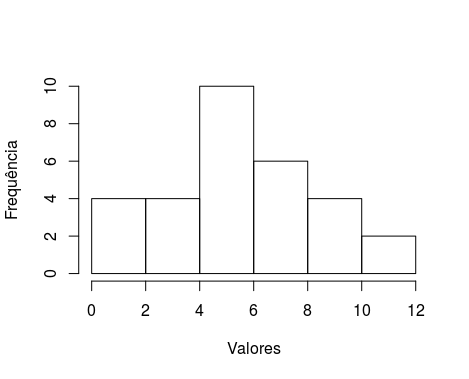
\includegraphics[scale=0.5]{histograma1.png}
  }
  \subfloat[][inclinação à esquerda] {
  	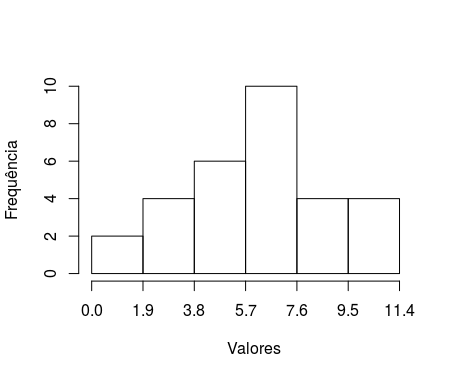
\includegraphics[scale=0.5]{histograma3.png}
  }
  \qquad % Quebra de linha
  \subfloat[][distribuição normal] {
  	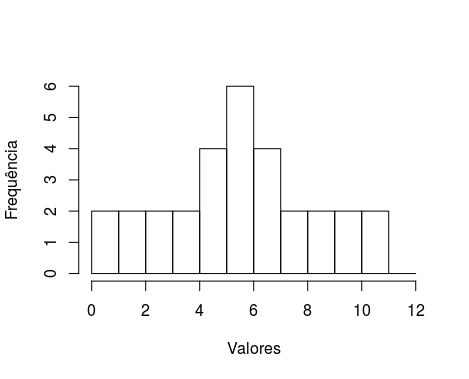
\includegraphics[scale=0.5]{histograma2.png}
  }
  \subfloat[][bimodal] {
  	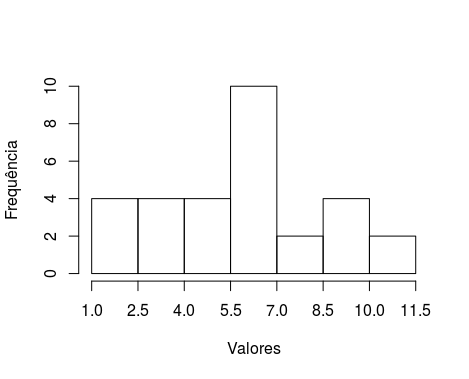
\includegraphics[scale=0.5]{histograma4.png}
  }    
  \caption{Histograma com diferentes fronteiras}
  \label{fig:exemplo-de-histograma}
  \source{Elaboração do autor}
\end{figure}

As \textit{Estimativas de Densidade de Kernel} (Kernel Density Estimators - KDE) são usadas para contornar esses problemas e para obter uma estimativa suave e diferenciável~\todo{Ronie: Explicar pq é bacana que ela seja diferenciável} (ref). O exemplo da figura~\ref{fig:exemplo-de-kde-a} mostra uma distribuição de probabilidade estimada usando-se KDE para o mesmo conjunto de dados problemáticos apresentados acima.

\begin{figure}[ht]
  \centering
  \subfloat[][suavização satisfatória] {
    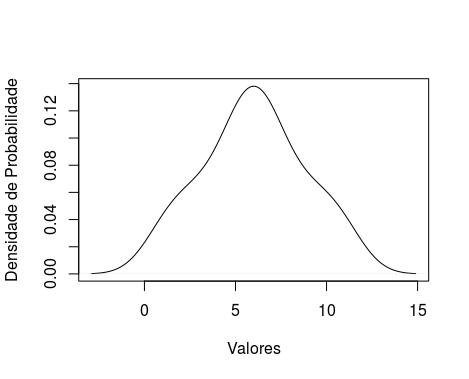
\includegraphics[scale=0.5]{densidade1.png}
    \label{fig:exemplo-de-kde-a}
  }
  \qquad % Quebra de linha
  \subfloat[][suavização em excesso] {
  	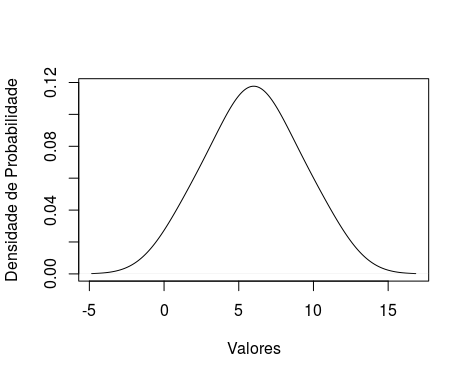
\includegraphics[scale=0.5]{densidade2.png}
  }
  \subfloat[][suavização insuficiente] {
  	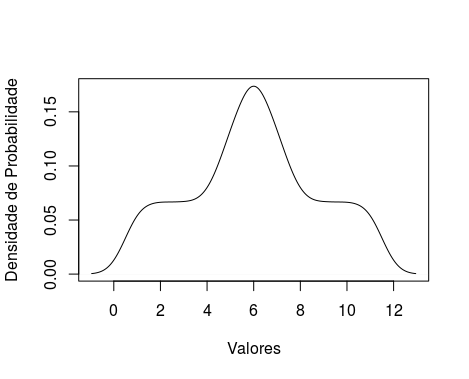
\includegraphics[scale=0.5]{densidade3.png}
  }    
  \caption{KDE com diferentes suavizações}
  \label{fig:exemplo-de-kde}
  \source{Elaboração do autor}
\end{figure}

As KDEs são usadas nesse trabalho principalmente nas análises salariais e tempo de permanência na ocupação. A distribuição dos salários segue o formato de pirâmide (ref) com muitos profissionais ganhando pouco e poucos profissionais ganhando muito. A análise gráfica da distribuição permite identificação de um certo \enquote{perfil salarial} e identificar pontos onde possa existir um fator que cause uma mudança significativa no salário.

A figura~\ref{fig:exemplo-de-kde-salario} exemplifica o que foi chamado \enquote{perfil salarial}, é possível identificar no gráfico que o salário para Recepcionista e Vendedor se concentram em torno de R\$ 1.000,00, porém Vendedores conseguem alcançar salários maiores, mas eles cessam abruptamente próximos aos R\$ 4.000,00.~\todo{Ronie: Trocar para cargos do cluster de Computação}

O KDE é um estimador de função de densidade de probabilidade, ou seja, ele cria uma estimativa da distribuição de probabilidade. Intuitivamente, ele pode ser compreendido como uma soma de pequenas distribuições. Partindo da suposição que cada valor observado poderia variar de acordo com uma distribuição normal, mas com o centro exatamente no ponto da observação, ao se somar todas essas \enquote{pequenas distribuições}, obtem-se uma estimativa da distribuição como um todo.

Em termos mais precisos, assumindo que o conjunto de valores observados $\boldmath{x} = (x_1, x_2, \ldots, x_n)$ foi extraído de uma distribuição desconhecida $f$, chamamos de $\hat{f}$ a função que é a estimativa de $f$. Essa estimativa é dada pela equação~\ref{eq:kde}.

\begin{equation} \label{eq:kde}
\hat{f}(\boldmath{x}) = \frac{1}{n}\sum_{i=1}^{n}{K_h(x - x_i)}
\end{equation}

Onde $K$ é a função de kernel e $h$ é o parâmetro de suavização conhecido como \textit{largura de banda} (bandwidth). Quanto maior $h$ mais suave é a função. A função kernel pode ser uma entre várias: Epanechnikov, Gauss, uniforme, etc. Uma opção comum, que condiz com a explicação intuitiva acima, é o uso da função de densidade de probabilidade normal, ou seja, uma curva de Gauss onde o pico (média) está em $x_i$ e a variância é $h$.

O KDE é sensível ao parâmetro de suavização, um valor muito alto esconde a distribuição real e um valor muito baixo cria picos artificiais que dificultam a análise visual. Várias propostas existem para se encontrar um valor ótimo para a largura de banda, como em \citeonline{Silverman1986-mv}, \citeonline{Sheather1991-su} e \citeonline{Scott1992-bd}. Uma opção exploratória, no entanto, é produzir diversos gráficos com larguras de bandas diferentes como demonstrado na figura~\ref{fig:exemplo-de-kde-gradiente}.

\begin{figure}[ht]
  \centering
  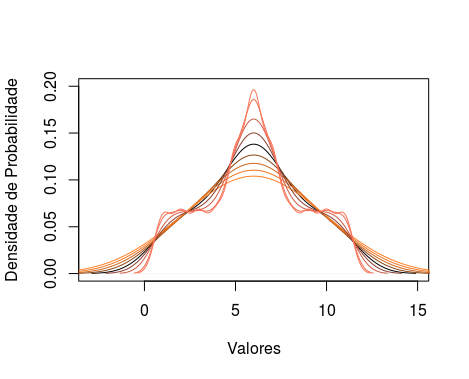
\includegraphics[scale=0.8]{densidade4.png}
  \caption{Densidade com diversas suavizações}
  \label{fig:exemplo-de-kde-gradiente}
  \source{Elaboração do autor}
\end{figure}

Pode-se resolver isso experimentalmente ou utilizando a técnica de \textit{Árvore de Modas} (Mode Tree) (ref)\ldots

\begin{figure}[ht]
  \centering
  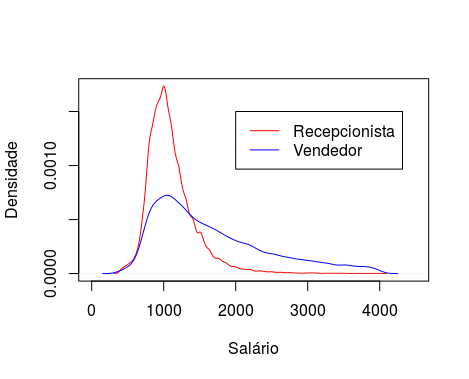
\includegraphics[scale=1]{salario_recepcionista_vendedor.png}
  \caption{Densidade de salários de recepcionista e vendedor}
  \label{fig:exemplo-de-kde-salario}
  \source{Elaboração do autor}
\end{figure}

As técnicas descritas até o momento são aplicáveis a análises univariadas, ou seja, baseadas em apenas um atributo. Também é interessante o uso de técnicas exploratórias para análises multivariadas, em que mais de um atributo é usado.

\textit{Gráficos de Dispersão} (Scatter Plots) são simples de serem criados e permitem uma noção visual da correlação ou agrupamentos entre dois atributos.

Esse gráfico é obtido usando o eixo $x$ para um atributo e o eixo $y$ para outro. Para cada registro, um ponto é colocado na intersecção entre os dois atributos. O desenho de uma matriz de gráficos de dispersão, onde cada um apresenta a correlação entre dois atributos permite a inspeção visual de várias correlações simultaneamente.

\begin{figure}[ht]
  \centering
  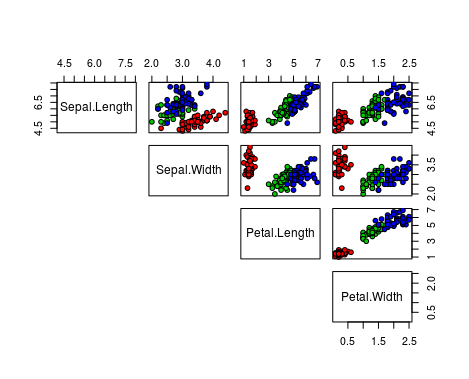
\includegraphics[scale=1]{scatterplot_matrix.png}
  \caption{Matriz de gráficos de dispersão}
  \label{fig:exemplo-de-matriz-de-dispersao}
  \source{Elaboração do autor usando os dados clássicos de \citeonline{Anderson1936-zq}}
\end{figure}

A figura~\ref{fig:exemplo-de-matriz-de-dispersao} é um exemplo de matriz de gráficos de dispersão usando um clássico conjunto de dados~\todo{Ronie: Trocar para idade vs salário de analista de sistemas}. As caixas na diagonal possuem os atributos e a intersecção entre cada uma apresenta o gráfico de dispersão entre os dois atributos. Nesse exemplo, os pontos de intersecção são coloridos com as classes dos objetos.

As correlações que aparecem visualmente no gráfico podem ser resumidas com estimadores como a \textit{Correlação de Pearson} ou a \textit{Correlação de Spearman}, entre outros. Contudo, a versão de Pearson é limitada a correlações lineares e a versão de Spearman, apesar de lidar trabalhar com correlações não lineares e não ser sensível a anomalias, pressupõe que a correlação seja monótona, ou seja, sempre crescente ou decrescente.

Essas limitações são contornáveis e com o uso do estimador correto obtêm-se uma informação confiável. Entretanto, a inspeção visual dos dados facilita essa escolha. De outra forma, os coeficientes de correlação precisam ser aplicados em um processo de tentativa e erro na busca por algum que possivelmente revele uma correlação.

\subsubsection{Agrupamento}

A ser definida.

\subsubsection*{Markov Clustering Algorithm}

A ser definida.

\subsubsection{Validação do Conhecimento}

A ser definida. [Checar \cite{Witten2016-vt}, parece que existe um capítulo dedicado a isso. Não tem =( é preciso procurar outras referências]

\subsubsection*{Validação Automática}

[TK Descrever métodos como validação cruzada e leave one out]

\subsubsection*{Validação Manual}

[TK Basicamente validação com um especialista e/ou por amostragem. Isso é importante pois algumas informações, principalmente as descritivas (como palavras relevantes e o agrupamento de carreira), são difíceis de validar só no automático]

A ser definida.

% ==========
\subsection{Grafos}

A movimentação entre uma ocupação e outra pode ser modelada como um grafo direcionado. Se um indivíduo passou de Programador para Analista de Sistemas, isso pode ser modelado como na figura X.

\question[inline]{Ronie: Eu deveria explicar conceitos básicos de grafo? Ou só como as informações do mapa estão organizadas (acho que isso iria para metodologia)?}

\subsubsection*{Vértices, Arestas, Atributos}

A ser definida.

\subsubsection*{Ciclos, Autorreferência, Cliques}

A ser definida.

% ==========
\subsection{Estatística Robusta e Estatística Não-Paramétrica}

A estatística robusta busca por estimadores equivalentes aos da estatística clássica, porém, menos sensíveis a anomalias e que sejam representativos mesmo quando a distribuição dos dados diverge significantemente da curva normal (ref.).

Nesse trabalho, estimadores robustos são importantes pois o banco de dados possui poucos filtros quanto a entrada de dados. Por exemplo, uma Faxineiro pode ter inserido, erroneamente, R\$ 12.000,00 como salário, enquanto que pelo mesmo motivo, um Diretor de Informática pode ter inserido R\$ 1.200,00 como salário. Mesmo retirando-se anomalias óbvias, existem dados ruidosos que não podem ser eliminados, mas distorcem as análises. O uso de estimadores robustos torna a análise menos suscetível a esse tipo de problema.

Um estimador resistente a anomalia tem pouca ou nenhuma variação na presença de dados com valores extremos. O estimador é tão mais \enquote{robusto} quanto mais valores extremos puderem ser inseridos na amostra sem que ele varie significantemente.

O equivalente robusto para o estimador de centralidade é a mediana ao invés da média. Por exemplo, em uma pequena amostra de cinco números: 10, 10, 10, 10, 1.000, a mediana aponta o número 10 como estimativa de centralidade, enquanto a média aponta para 208.

O \textit{ponto de quebra} (breakpoint) da mediana é de 50\%, ou seja, é preciso que metade da amostra esteja \enquote{contaminada}~\footnote{Por contaminação entenda-se um valor extremo indevido na amostra} para que ele altere significantemente seu valor. Já no caso da média, um único valor extremo causa essa alteração.

Algumas técnicas são usadas para que estimadores da estatística clássica se tornem mais robustos, como \textit{trimmed estimators} e \textit{Winsorised estimators} [TK achar tradução e adiciona explicação].

Já a estatística paramétrica trata de métodos que são equivalentes ao da estatística clássica, mas que não assumem um modelo de distribuição de probabilidade~\cite{Hollander2013-mq}. Ou seja, ela possui a propriedade de ser \textit{independente de distribuição} (distribution-free). 

Nesse trabalho, a estatística não paramétrica é empregada pois poucos dados seguem uma distribuição normal clássica. Por exemplo, os salários são similares à ela, mas com diversas inclinações à direita e com grande variedade na acentuação da inclinação. Também não é incomum que a distribuição seja multimodal, ou seja, possua vários picos. Dessa forma, análises que não assumem uma distribuição normal (ou conhecida) permitem uma análise mais rápida, já que não é necessária a aplicação de técnicas para torná-la uma normal; e mais confiável, já que, no caso desse trabalho, o modelo da distribuição é uma das características a ser descoberta.~\todo{Ronie: Acho que posso ficar só com isso, faz todo o sentido já que não }

As estatísticas robustas e não-paramétricas são particularmente úteis para a análise exploratória por não necessitarem de modelos previamente assumidos ou de tratamentos especiais para anomalias. Assim, não é preciso criar uma fase de pré-análise exploratória para validar os modelos de distribuição nem detectar as anomalias. A análise exploratória pode indicar as melhores abordagens para essas tarefas. 

Os métodos descritos no capítulo \ref{sec:analise-exploratoria} são métodos robustos e não-paramétricos.

% ==========
\subsection{Mapa de Carreiras}

O Mapa de Carreiras (MCar) traz o resumo da trajetória profissional de cerca de 10 milhões de pessoas e uma de suas manifestações pode ser vista no site http://www.vagas.com.br/mapa-de-carreiras. Internamente, essas informações estão armazenadas em um banco de grafos e são periodicamente atualizadas. Nesse grafo, os vértices representam \textit{ocupações} e as arestas representam as \textit{migrações} entre ocupações. O grafo do MCar foi gerado a partir do histórico profissional dos currículos do site de carreiras VAGAS.com desde 2011. São cerca de 23 milhões de históricos profissionais.\footnote{Leandro: ... PRECISAREMOS INTRODUZIR ALGUNS CONCEITOS SOBRE GRAFOS (SUBSEÇÃO ACIMA). Ronie: seção adicionada, escrevendo.}

[TK Falta referência para o gráfico]

\begin{figure}[ht]
  \centering
  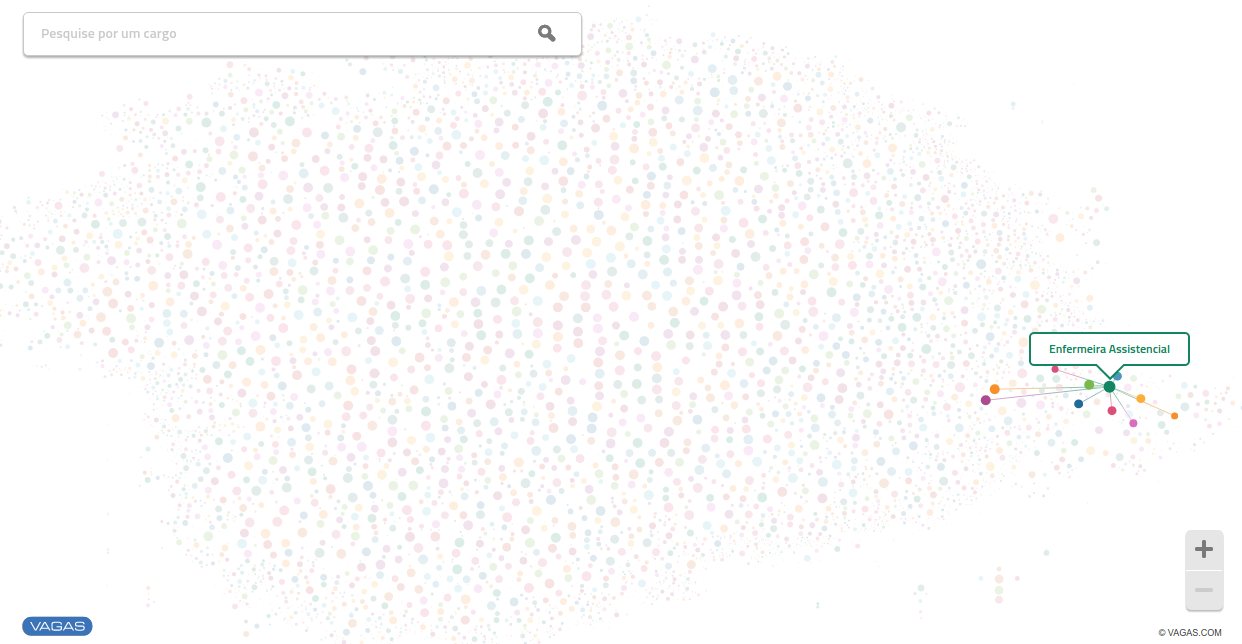
\includegraphics[scale=0.3]{Grafo_Enfermeira_Assistencial.png}
  \caption{Exemplo do Grafo de Ocupações}
  \label{fig:exemplo-grafo}
\end{figure}

No contexto do Mapa de Carreiras, uma \textit{ocupação} significa uma atividade profissional, remunerada ou não. A maior parte dessas ocupações são profissões remuneradas, tais como \enquote{Babá} ou \enquote{Arquiteto}, entretanto, algumas delas aparecem como atividades principais de uma pessoa, mas não necessariamente uma profissão, tais como: \enquote{Mestrando}, \enquote{Enfermeiranda} ou \enquote{Voluntário}. Os vértices possuem diversos atributos que são resumos estatísticos daquela ocupação. Em específico, possuem o número de pessoas atualmente exercendo a profissão, a distribuição salarial e a distribuição do tempo de permanência em uma ocupação, entre outras.

As arestas que conectam as ocupações representam \emph{migrações} entre elas, ou seja, o fluxo de pessoas que exercia uma cerca ocupação e passou a exercer outra. Acompanhar as arestas permite observar o movimento dos profissionais no mercado de trabalho. O principal atributo das arestas é o número de profissionais que fizeram a trajetória de uma ocupação para outra.

[TK Falta referência para o gráfico e poderia limpar o canto esquerdo]

\begin{figure}[ht]
  \centering
  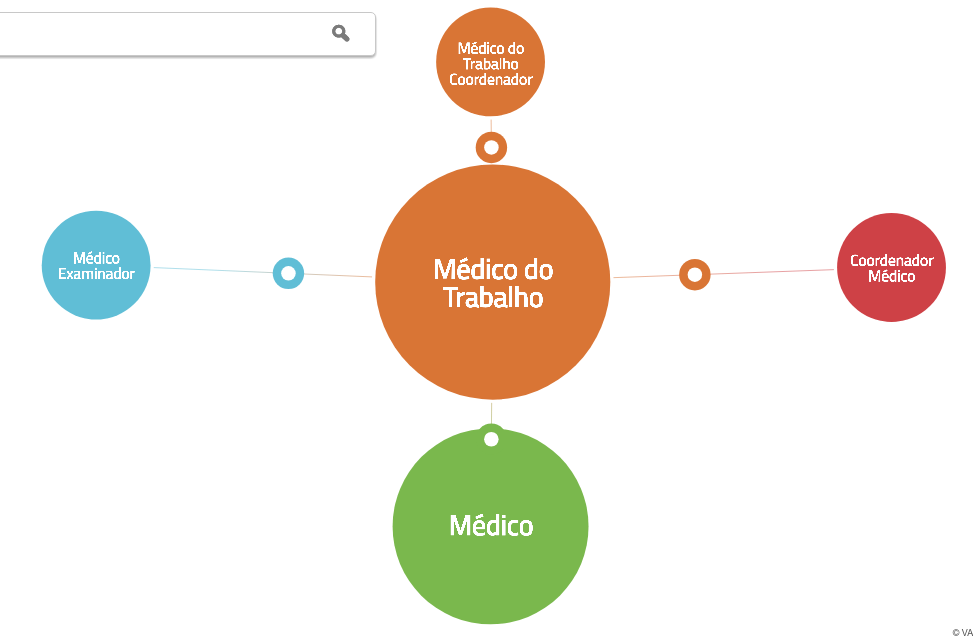
\includegraphics[scale=0.3]{Grafo_Medico_do_Trabalho.png}
  \caption{Ocupações próximas a Médico do Trabalho}
  \label{fig:exemplo-medico-do-trabalho}
\end{figure}

O grafo do MCar é direcionado e, portanto, o fluxo de migração entre ocupações possui uma direção específica, mas é comum existir migração em ambos os sentidos entre duas ocupações. No grafo, esse movimento é representado por duas arestas diferentes, mesmo que visualmente exista uma única aresta. Em outras palavras, o MCar é um grafo direcionado com ciclos, porém os vértices não são autorreferentes. \footnote{Leandro: MAS É POSSÍVEL QUE ALGUÉM RETORNE A UMA OCUPAÇÃO ANTERIOR APÓS ALGUM TEMPO E ISSO FORMARIA UM CICLO, CERTO? NOTE QUE O LAÇO NÃO APARECE APENAS EM UMA MIGRAÇÃO DE ALGUÉM PARA SI MESMO. Ronie: Texto Ajustado}

Por causa desses ciclos, não é possível criar uma ordenação topológica que represente um clara progressão de carreira. Entretanto, é possível extrair grupos de ocupações que possuem migrações mais frequentes entre si. Esses agrupamentos são comumente acíclicos, o que possibilita traçar essa progressão entre as ocupações que o compõem. Nos experimentos do capítulo XX é possível observar que essa característica é mais frequente observada em grupos formados por ocupações que requerem maior qualificação técnica, como \enquote{Comércio Exterior}. Já nas ocupações ditas \enquote{operacionais}, o fluxo de movimentação entre ocupações acentua a característica cíclica do grafo. Particularmente, é possível observar um forte ciclo entre as ocupações \enquote{Recepcionista}, \enquote{Vendedor} e \enquote{Auxiliar Administrativo}.\footnote{Ronie: Adicionei esse parágrafo para expandir um pouco a ideia do ciclos. Essa parte é realmente interessante em uma análise do mercado de trabalho: não existe uma progressão clara para trabalhos operacionais, já trabalhos que exigem mais conhecimento possuem claramente o conceito de progressão, culminando frequentemente em cargos administrativos. Por outro lado, quebrou um pouco o fluxo do texto.}

Para a construção dos vértices, os textos presentes nos títulos dos históricos profissionais dos currículos foram \enquote{normalizados}. Nesse contexto, \enquote{normalização} significa transformar os títulos com o mesmo significado na mesma representação textual. Por exemplo, a mesma ocupação pode ter sido registrada por pessoas diferentes como \enquote{Moto Boy}, \enquote{moto boy}, \enquote{Motoboy}, \enquote{Moto Girl} entre outras variações. O que chamamos de \enquote{normalização} é o trabalho de transformar essas diferentes grafias em uma única que possa ser usada para identificação da ocupação. No caso, todas as anteriores são normalizadas para \enquote{motoboy}. Esse trabalho também inclui a correção ortográfica e a remoção de abreviação das ocupações. \footnote{Leandro: SEU TRABALHO VAI EXIGIR UMA BASE CONCEITUAL DE MINERAÇÃO DE TEXTOS NA QUAL FALAREMOS DE TODAS AS PRINCIPAIS ETAPAS DE PREPARAÇÃO DE TEXTOS, ENFOCANDO AQUELAS USADAS NA SUA PESQUISA. Ronie: Introduzida uma seção acima para falar sobre isso}

Após a normalização são criados pares de ocupações cronologicamente ordenados. Isso significa que o término de uma ocupação precisa coincidir com o início da seguinte. Uma margem de um mês de tolerância na sobreposição corrige pequenas imprecisões na anotação dos históricos profissionais. Currículos com apenas uma ocupação são descartados, bem como ocupações que se sobreponham cronologicamente ou que estejam separadas por um intervalo de tempo maior que um ano.

Os pares de ocupações são unificados produzindo as arestas e os vértices, o grafo é então podado das arestas menos relevantes. Arestas com menos de dez migrações são removidas do grafo e vértices desconectados depois desse processo são removidos. Esse critério de poda foi definido empiricamente através de análise por amostragem. Números muito maiores removiam vértices e migrações relevantes de ocupações mais especializadas como \enquote{Comandante} ou \enquote{Engenheiro de Minas}, enquanto números muito menores acrescentavam vértices espúrios causados por erros de grafia que a fase de correção ortográfica foi incapaz de detectar.

Um dos efeitos indesejados desse processo é que algumas ocupações legítimas são removidas do grafo. É o caso de ocupações muito recentes, muito especializadas ou que ainda não possuem uma concordância da nomenclatura entre os profissionais da área. Como exemplo podemos citar \enquote{Especialista em Experiência do Usuário}, uma profissão recente, que também é chamada \enquote{Analista de UX} ou apenas \enquote{UX}.

Duas outras limitações no grafo ocorrem por conta da experiência profissional ser um campo de texto livre, ou seja, o usuário digita livremente sua ocupação sem estar restrito a uma lista de opções. A primeira se refere a vértices que representam uma ocupação dupla, como \enquote{Caixa e Balconista} ou \enquote{Atendente/Estoquista}. A segunda ocorre por ambiguidade no nome da ocupação, como \enquote{Coordenador de Projetos}, que ocorre na carreira de Desenvolvimento de Software e na de Engenharia Civil.

Por outro lado, o campo de texto livre permite a captura de ocupações que pouco provavelmente apareceriam em uma lista curada, como \enquote{IRLA} (Instalador Reparador de Linhas Aéreas) ou \enquote{Rigger} (pessoa no solo que orienta o posicionamento de carga para o operador de guindaste).

Ao final do processo o grafo possui cerca de 8.348 ocupações distintas e 14.031 arestas. Esses números flutuam dependendo das atualizações dos currículos em que são baseados e no crescimento natural do banco de dados. Os dados presentes nesse trabalho refletem a base atualizada em Fevereiro de 2017.

\section{METODOLOGIA} \label{sec:metodogia}

\todo[inline]{Está havendo uma grande modificação nos rumos do trabalho. O começo do capítulo até que está \enquote{ok}, mas dali a pouco a coisa fica esquisita :(}

% Parte inserida depois da última revisão. Muito, muito controversa se essa linha de trabalho vai ser mantida.
Esse projeto de pesquisa se propõe a criar um sistema capaz de executar continuamente diversas análises sobre os dados de currículos, fornecendo um retrato atualizado constantemente do mercado de trabalho.

O sistema possui duas grandes etapas. A primeira extrai os currículos de um banco relacional e os condensa para formar um mapa de movimentação de pessoas entre as ocupações. A segunda usa os currículos e o mapa para gerar duas informações: quais atributos estão associados à mudança no perfil salarial e qual a próxima ocupação provável para um certo indivíduo, dado seu currículo atual.

% Fim da parte inserida

%Esse trabalho consiste em um sistema que extrai dados de um banco de dados relacional e os organiza em um banco de grafos. Pelos motivos explicados a seguir, uma vez montado, esse processo precisa ser executado com o mínimo de intervenção manual.~\todo{Leandro: REMOVER}

%Novos currículos entram diariamente e fornecem dados que podem aprimorar a qualidade dos resultados. Por esse motivo, deve-se ser capaz de reexecutar a análise constantemente.

\todo[inline]{Leandro: REMOVER. A IDEIA É ESTRUTURARMOS O GRAFO E TRABALHARMOS NA SUA VERSÃO ESTÁTICA. O GRAFO DINÂMICO FICA PARA TRABALHOS FUTUROS}

%O processo como um todo pode ser aprimorado em vários pontos. Novas análises podem ser introduzidas, análises anteriores podem ser modificadas e refinadas. Portanto, cada componente do processo deve ser facilmente alterável. Por \enquote{facilmente alterável}, compreende-se que alterações provocam pouco ou nenhum retrabalho e que não afetem o sistema para além do componente onde foi feita.~\todo{Leandro: REMOVER}

\subsection{Os Dados}

Os dados fonte para essa pesquisa são currículos anonimizados de usuários do site de carreiras VAGAS.com.br. Esses currículos são armazenados em um banco de dados \textit{Microsoft SQL Server}. No total há cerca de 10 milhões de currículos armazenados entre 1999 e 2016, mas para esse trabalho apenas os currículos atualizados entre 2011 e 2016 serão utilizados. % FALE AGORA DOS CVS DA ÁREA DE TECNOLOGIA. QUANTOS SÃO? QUANTAS E QUAIS SÃO AS CARREIRAS (A LISTAGEM DAS CARREIRAS PODE VIR COMO UM APÊNDICE)

Para o processamento das análises a serem explicadas nesse capítulo, os dados serão primeiramente extraídos para arquivos textos e só então processados. Cada registro é colocado em formato JSON (\textit{Javascript Object Notation}) e ocupa uma linha do arquivo texto, cada linha contém apenas um registro. % E QUAL É O CONTEÚDO DE CADA REGISTRO?

Optou-se por essa abordagem pois o banco SQL Server é responsável pela operação da empresa e consultas pesadas poderiam afetá-la indevidamente. Outra razão para essa opção se baseia no método de acesso aos dados durante o processamento da informação, os dados são lidos sequencialmente por todos os processos, dispensando a necessidade de um mecanismo de acesso a dados de forma arbitrária, como consultas SQL.

\subsection{O Processamento da Informação}

A arquitetura para o sistema de processamento da informação deve ser capaz de atender às necessidades de \textit{repetibilidade}~\todo{Melhorar nome} e \textit{modificabilidade} descritas no início do capítulo~\ref{sec:metodogia}. O sistema também deve ser escalonável horizontalmente, significando que seja possível acrescentar mais máquinas para acelerar o processamento ao invés da opção do emprego de máquinas de maior porte. Dessa forma, o aumento no volume dos dados ou na quantidade de processamentos pode ser absorvido pelo sistema sem que grandes investimentos sejam feitos. % NUMA LINHA DE SISTEMAS INTELIGENTES ESSA DISCUSSÃO SOBRE ESCALONAMENTO HORIZONTAL NÃO É CENTRAL AO TRABALHO. A QUAL PROCESSAMENTO DE INFORMAÇÃO VOCÊ SE REFERE AQUI?

O padrão arquitetural que atende aos requisitos acima é conhecida como \textit{Pipes and Filters}~\cite{Hohpe2003-nj}, \textit{Dataflow}, \textit{Stream Processing} ou \textit{Flow Based Programming}~\cite{Morrison2010-pm}. Nesse padrão, os dados fluem continuamente de um processo para o outro, sendo transformados e filtrados conforme o processo avança\todo{Ronie: FBP no referencial teórico}. 

Como cada processo trabalha um registro de cada vez, evitando carregar todos os dados em memória, ele consome memória apenas o suficiente para os registros que estão em processamento no momento. Assim, uma única máquina trabalha volumes de dados muito maiores do que sua memória RAM disponível (ref). Adicionalmente, os processos podem ser executados paralelamente em um mesmo computador ou distribuídos por diversas máquinas, possibilitando que o tempo de processamento diminua se comparado ao uso de apenas um processador ou computador. Por outro lado, a transmissão de dados via rede entre computadores é um processo comparativamente lento em relação ao acesso direto em memória (ref quanto?). Para que o uso distribuído seja de fato mais rápido, é preciso que a transferência de dados entre computadores seja a menor possível e o trabalho executado por cada um seja o maior possível.

% ATÉ AGORA AINDA NÃO ESTOU CERTO DA NECESSIDADE DESSES PARÁGRAFOS ACIMA. HÁ UM ASPECTO IMPORTANTE DE SEU TRABALHO QUE AINDA NÃO ESTÁ ESCRITO QUE É O FOCO DA PESQUISA. POR EXEMPLO, NA SEÇÃO QUE DESCREVE OS DADOS ACIMA, EU ESPERARIA UMA DESCRIÇÃO DO QUE SÃO OS DADOS QUE SERÃO USADOS PARA CONSTRUIR OS GRAFOS DE CARREIRA, INCLUINDO UM PEQUENO EXEMPLO ILUSTRATIVO. ESSA PART DE PROCESSAMENTO DA INFORMAÇÃO AINDA NÃO CAIU A FICHA PRA MIM.

Em uma estrutura de \textit{pipeline}, cada processo possui apenas uma interface de entrada e uma interface de saída. Desde que mantenha a mesma interface, um processo pode ser substituído por outro, ou por um conjunto deles, sem afetar outras partes do sistema. Isso permite que ajustes e novos experimentos sejam feitos de maneira bastante simples se comparados a arquiteturas com maior número de componentes que interagem entre si, como \textit{Actor Model} ou \textit{Arquiteturas Orientadas a Objetos}.

É possível compor novos \textit{pipelines} reutilizando partes de outros \textit{pipelines}. É possível observar esse reuso na descrição dos pipelines em seções posteriores.

Essa arquitetura foi implementada em máquinas \textit{Linux} utilizando \textit{pipes} e \textit{sockets} para comunicação interprocessos. Um \textit{pipe} no \textit{Linux} é uma implementação de FIFO em memória RAM. A informação é gravada na fila exatamente como seria em um arquivo. Do outro lado um outro processo lê da fila da mesma forma. Por usar a mesma interface que leituras e gravações em arquivo, qualquer programa capaz de executar essas operações pode ser usado como parte do \textit{pipeline}.

\textit{Sockets}, por sua vez, abstraem a transferência de dados entre processos ou computadores através de uma interface padronizada. Ao invés dos \textit{sockets} nativos do \textit{Linux}, optou-se pelo \textit{ZeroMQ} que é uma implementação mais robusta, criada para transmissão de dados em diversos modelos de distribuição~\cite{Hintjens2013-tz}.

O \textit{ZeroMQ} possui interfaces para diversas linguagens de programação, mas para preservar a interface entre processos foram criados componentes que traduzem a entrada em \textit{pipes} para \textit{sockets ZeroMQ} e vice-versa.

O uso de JSON como formato de dados e o uso de \textit{pipes} foram escolhidos para que programas e linguagens diversas possam interoperar. Dessa forma, o leque disponível de ferramentas não se restringe às opções disponíveis em uma única linguagem de programação.

A maior parte dos processos foi implementada em Ruby. Apesar de não ser uma linguagem reconhecida pela sua velocidade, ela possui capacidades importantes para esse trabalho. Para os processos que consistem em modificação de texto, com limpeza e normalização, a linguagem possui um processador de expressões regulares com capacidades avançadas, chamado \textit{Onigmo}. Por ser uma linguagem interpretada, não há etapas de compilação, por ser uma linguagem de alto nível, não são necessários cuidados com liberação de memória e representação dos dados em detalhes. Adicionalmente, é uma linguagem com uma grande quantidade de bibliotecas prontas para as mais diversas tarefas, são cerca de 8.000 bibliotecas no repositório oficial do Ruby, o Rubygems~\cite{rubygems-ud}; essas características possibilitam um ciclo mais rápido de escrita e testes de componentes se comparado com linguagens sem essas propriedades.

Com características similares às mencionadas, a linguagem Python seria outra candidata igualmente viável para a implementação do projeto. O fator decisório, nesse ponto, foi a familiaridade do pesquisador com a linguagem Ruby. É esperado que essa familiaridade diminua a chance de erros operacionais e acelere a escrita de componentes, permitindo que mais explorações sejam feitas no mesmo tempo.

Ainda assim, durante a construção, alguns processos foram implementados em Python e R para explorar técnicas disponíveis em bibliotecas dessas linguagens, entretanto, esses componentes não fizeram parte da versão final\todo{Por exemplo, \enquote{stemming}, que não foi usado}. Alguns outros processos usam programas específicos como o MCL para agrupamento de ocupações e o Graphviz para distribuição do grafo em um plano bidimensional para visualização.

Os componentes que se tornam gargalos do sistema são reimplementados em Rust para melhor desempenho. Rust é uma linguagem com velocidade similar a do C, mas com mecanismos específicos para evitar problemas com manipulação de memória~\cite{rustfaq-ys}.

As análises são feitas pelos \textit{pipelines} descritos a seguir.

% EM PRINCÍPIO QUASE TODA ESSA DESCRIÇÃO ACIMA É DESNECESSÁRIA PARA EFEITOS CIENTÍFICOS. VEJAMOS ADIANTE COMO VOCÊ PROGRIDE E A GENTE DECIDE O QUE FAZER COM ESSA SEÇÃO QUE TERMINA AQUI

\subsection{Montagem do Grafo} \label{sec:montagem-grafo}

Esse \textit{pipeline} responsável por montar um grafo onde os vértices representam ocupações e as arestas representam o fluxo de pessoas cuja trajetórias profissionais passou por essas ocupações.

Ele inicia com a extração de dados do banco de dados relacional, passa por processos de limpeza, agrupamento e finaliza com a gravação do resultado final em um banco de grafo.

O \textit{pipeline} é exibido na figura~\ref{fig:montagem-do-grafo}.

\begin{figure}[ht]
  \centering
  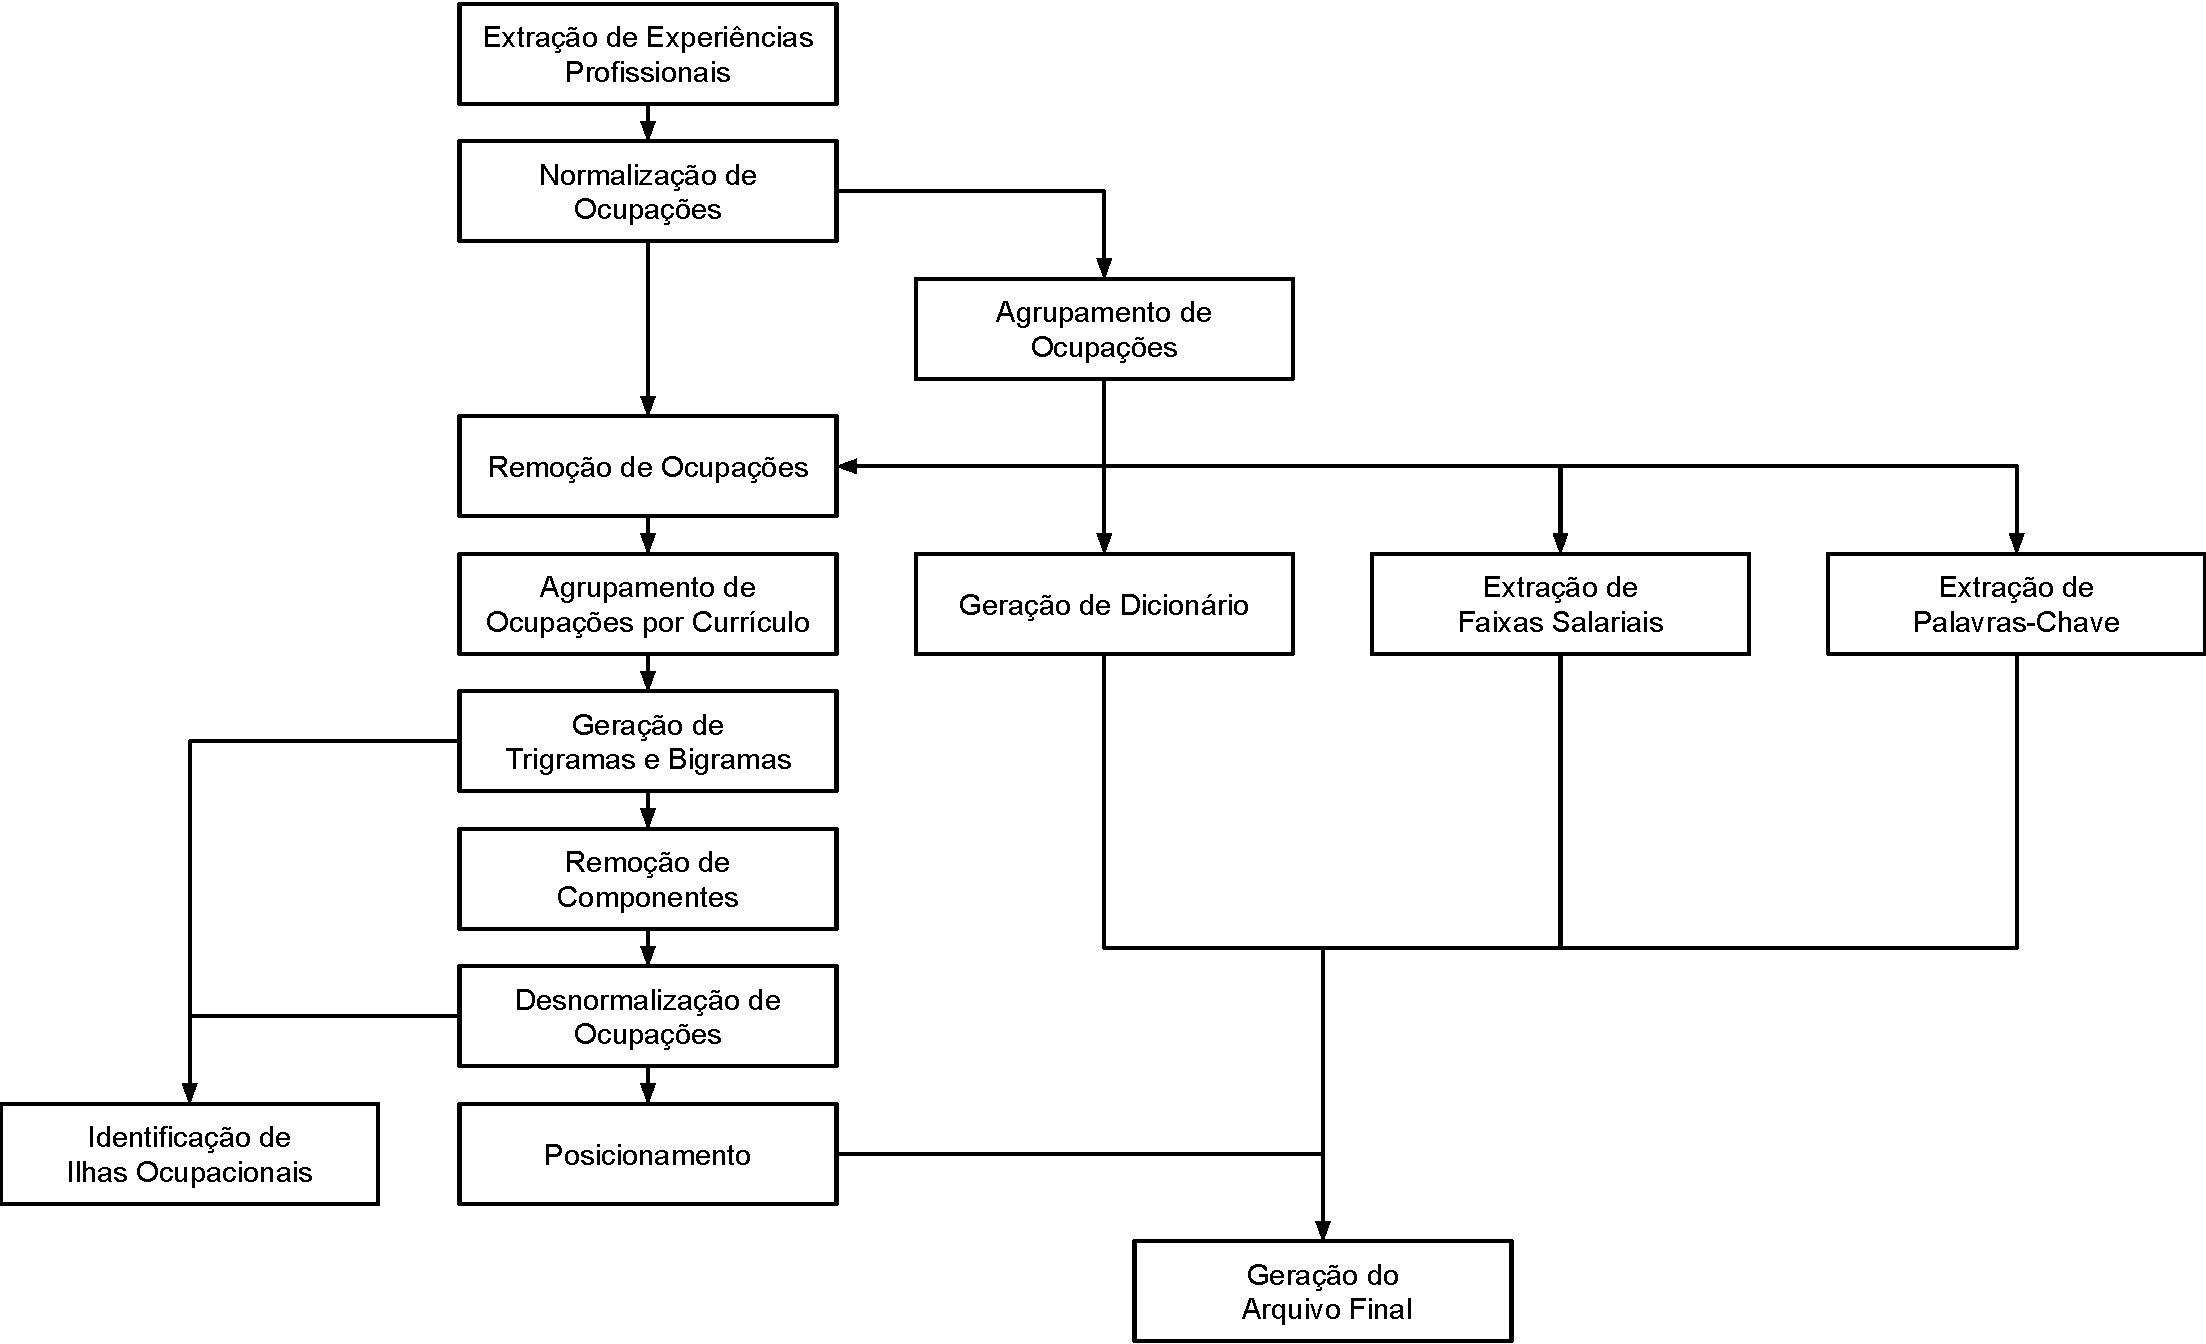
\includegraphics[scale=0.4]{pipeline1.pdf}
  \caption{Montagem do Grafo}
  \label{fig:montagem-do-grafo}
\end{figure}

\subsubsection{Extração do Experiências Profissionais} \label{sec:extracao-experiencia}

O primeiro processo do \textit{pipeline} extrai os banco de dados relacional e os grava em arquivos textos para processamento posterior. O processo principal não extrai currículos, mas sim experiências profissionais. Cada registro representa uma única experiência.

Os dados extraídos são:

\begin{itemize}
\item Identificador do Currículo
\item Nome da Ocupação
\item Data de Início
\item Data de Término
\item Texto Descritivo
\end{itemize}

O \textit{Identificador do Currículo} é um número único para cada currículo dentro do banco de dados.

O \textit{Nome da Ocupação} é o texto digitado livremente pelo usuário no campo nomeado \enquote{Cargo} no currículo.

As \textit{Data de Início} e \textit{Data de Término} marcam quando o profissional iniciou naquela ocupação e até quando a exerceu. Se é a ocupação atual, não existe uma data de término.

O \textit{Texto Descritivo} é o texto digitado livremente pelo usuário no campo com o nome \enquote{Descrição} no currículo.

Quando uma atualização de dados precisa ser feita, esse processo lê novamente do banco de dados. Se a atualização não é necessária, esse processo lê do arquivo previamente gravado e alimenta o processo seguinte.

\subsubsection{Normalização de Ocupações} \label{sec:normalizacao}

Nessa etapa, o nome da ocupação é normalizado para uma classe de maneira que todas as grafias que signifiquem a mesmo ocupação sejam transformadas na mesma classe. Nesse trabalho, essa classe é chamada \enquote{classe equivalente} ou \enquote{ocupação normalizada}.

Para transformar o texto digitado em uma ocupação normalizada os erros de digitação são corrigidos, pontuações são removidas, abreviaturas frequentes são expandidas, o texto é colocado em caixa baixa, é feita a singularização das palavras que compõem a ocupação e os nomes são masculinizados (\enquote{secretária} se transforma em \enquote{secretário}, por exemplo).

Ocupações com múltiplas palavras também são ordenadas alfabeticamente. Dessa forma, ocupações como \enquote{Auxiliar Financeiro-Administrativo} e \enquote{Auxiliar Administrativo-Financeiro} resultam na classe \enquote{administrativo auxiliar financeiro}.

As classes resultantes lembram vagamente o termo original, como no exemplo anterior, em um processo posterior, é criado um dicionário entre a classe equivalente e um nome que tenha significado para o usuário.

\subsubsection{Remoção de Ocupações pouco Frequentes}

Mesmo com o processo de correção e normalização, algumas experiências profissionais estão escritas de maneira única. Isso pode significar um erro, uma ocupação singular ou o uso de termos pouco convencionais, como o objetivo da pesquisa é desenhar carreiras \enquote{comuns}, os casos únicos podem ser seguramente removidos sem a necessidade de distingui-los.

\subsubsection{Remoção de Ocupações Incorretas}

Mesmo após a remoção de casos únicos, alguns nomes presentes nesse campo não podem ser realmente considerados "ocupações". São erros comuns que a etapa de normalização não foi capaz de corrigir ou representam um entendimento errôneo por parte do usuário.

Casos emblemáticos são ocupações que possuem o título \enquote{sim}, \enquote{não} ou \enquote{o mesmo}. Especialistas da empresa criaram manualmente um dicionário com os erros mais comuns. Esse dicionário foi aprimorado posteriormente à publicação do MCar com sugestões dos usuários.

\subsubsection{Agrupamento das Ocupações por Currículo}

As ocupações são agrupadas por currículo, formando uma sequência cronológica das experiências de um profissional.

\subsubsection{Remoção de Experiências sem Conexão ou Sobrepostas}

Como o objetivo final dessa etapa é criar um banco de grafos que sumarize o movimento de pessoas entre ocupações, as experiências profissionais que não se conectam cronologicamente com nenhuma outra são removidas. Intuitivamente, quanto maior a distância entre as experiências, menos provável é que elas sejam sequência natural da carreira e mais provável que sejam movimentos laterais ou que sejam regressões.

O benefício da grande quantidade de dados é que uma abordagem conservadora para situações como essa ainda deixa uma grande quantidade de dados para se trabalhar. Nesse ponto, optou-se por considerar desconexa quaisquer experiências sequenciais cujo início da posterior esteja a mais do dois meses de distância do fim da anterior.

Na mesma etapa, removem-se experiências profissionais que se sobreponham. Uma vez sobrepostas, não é possível afirmar que uma é sequência natural da outra ou que sequer tenham relação entre si. É comum encontrar no banco de dados carreiras paralelas em que gestores também são professores ou que técnicos também sejam voluntários. Da mesma maneira que experiências desconexas, as que se sobrepõem por mais de dois meses são removidas.

\subsubsection{Remoção de Currículos por Experiência}

Após o processo anterior, são removidos os currículos que possuam uma ou menos experiências profissionais.

\subsubsection{Geração de Pares de Experiência}

As experiências profissionais de cada currículo são pareadas por ordem cronológica. Por exemplo, um currículo que tenha a seguinte sequência de ocupações \enquote{Faxineiro \textrightarrow~Copeiro \textrightarrow~Chapeiro}, produz os pares \enquote{Faxineiro \textrightarrow~Copeiro} e \enquote{Copeiro \textrightarrow~Chapeiro}.~\question{Colocar em notação de conjunto?}

\subsubsection{Agrupamento de Pares de Ocupações}

Pares iguais de ocupações são agrupados e contados, gerando um \textit{multiset}. o número de repetições é anotado como uma propriedade de cada par único. A grosso modo, o número de repetições em um par representa o número de pessoas que migraram de uma ocupação para outra.

Os pares que saem ao final desse processo formam um grafo em formato textual. Diversos programas são capazes de trabalhar com um formato similar a esse, como o Graphviz ou o MCL.

As etapas posteriores podam o grafo em suas arestas menos relevantes e transformam sua representação textual para que possa ser lido por outros programas.

\subsubsection{Remoção de Pares Pouco Frequentes} \label{sec:grafo-final}

A maior parte dos pares de ocupações ocorrem pouquíssimas vezes. Em um conjunto com XX pares, cerca de XX ocorrem apenas uma vez. Esse pequeno número de repetições é causado tanto por trajetórias incomuns quanto por erros de digitação que as etapas anteriores não foram capazes de eliminar. Por vezes, são apenas ocupações similares a outras, mas onde os usuários escrevem de maneira pouco convencional. Com alguma frequência, os pares realmente representam trajetórias em carreiras extremamente específicas.

Para encontrar um número de corte foi feita uma avaliação manual por amostragem. Amostras com algumas centenas de pares com números de corte entre 1 e 30 foram analisadas por especialistas da empresa junto com o pesquisador. O objetivo foi encontrar um número que não fosse conservador demais, removendo trajetórias válidas, nem liberal demais, permitindo trajetórias com erro.

Após o processo de análise, chegou-se a um número próximo a 10 repetições. Pares de ocupações com menos de 10 repetições são removidos.

\subsubsection{Posicionamento dos Vértices do Grafo}

Para que o grafo possa ser exibido bidimensionalmente, é preciso que seus vértices sejam posicionados de modo a evitar a sobreposição.

É usado o algoritmo de \textit{Force-Directed}~\todo{Colocar o algoritmo Force-Directed no referencial teórico} para posicioná-los corretamente. Esse algoritmo é aplicado nesse passo utilizando o programa Graphviz.

A saída do Graphviz é um arquivo texto com a posição X e Y do vértice em um plano cartesiano. Os valores absolutos de X e Y não são relevantes pois o plano é comprimido ou expandido posteriormente para se adequar à tela do usuário do MCar.

\subsubsection{Descoberta de Proto-Carreiras}\todo{Título provisório e bem ruim}

O grafo gerado no passo~\ref{sec:grafo-final} é usado nesse processo para gerar agrupamentos de ocupações fortemente correlacionadas. Uma ocupação é correlacionada a outra se há um movimento migratório entre elas. No grafo, esse movimento migratório é representado pelo número de repetições anotadas em um par de ocupações.

Intuitivamente, os grupos formados por esse processo significam ocupações com maior migração entre si do que com outros grupos. Ou seja, em termos probabilísticos, um indivíduo tem maior chance de permanecer nesse grupo do que deixá-lo.

Entre duas ocupações, o fluxo de migrações indica uma certa preferência por uma das duas. Por exemplo, se o número de migrações entre \enquote{Analista da Sistemas \textrightarrow~Coordenador de Projeto} for maior que o reverso \enquote{Coordenador de Projeto \textrightarrow~Analista da Sistemas}, intuitivamente considera-se que \enquote{Coordenador de Projeto} é uma ocupação mais desejável do que \enquote{Analista de Sistemas}.

Dentro de cada grupo de ocupações, é possível notar que essa ordem de preferência vai normalmente de ocupações mais operacionais e com salários mais baixo para ocupações mais gerenciais e com salários mais altos. O que coincide com a noção comum de progressão de carreira.

A grosso modo, o agrupamento e o fluxo de migração das ocupações revela o que se pode considerar um \enquote{protótipo de carreira}. Ou seja, um esboço onde um indivíduo em uma ocupação desse grupo tem uma probabilidade maior de se manter nele e de migrar de onde estiver para as posições mais desejáveis no topo do grupo.

Existe, no entanto, um grupo digno de nota resultado desse processo. Ao se ordenar topologicamente~\todo{Colocar ordenação topológica no referencial teórico} esse grupo, não há uma ordem de preferência clara entre as ocupações, o que indica que não há uma noção de escalada como nos outros grupos. Ele também possui algumas ocupações que são \textit{hubs}~\todo{Explicar hub no referencial teórico, está em \enquote{redes complexas}} que conectam uma grande quantidade de outras ocupações.

Ao analisar manualmente o grupo, nota-se que ele é quase todo composto pelo que é comumente chamado \enquote{trabalho operacional}. A escolaridade mais frequente nessas ocupações é a de \textit{segundo grau completo}, isso significa que essas ocupações não necessitam de treinamento especializado para serem desempenhadas, o que reforça a crença que esse grupo reflete a própria definição de \enquote{operacional}.

Algumas outras ocupações também possuem \enquote{segundo grau completo} como escolaridade mais frequente, mas se comportam como os outros, com um divisão clara entre eles o outros e com uma direção de preferência entre as ocupações. Uma análise manual da descrição das suas ocupações e das palavras-chave relacionadas sugere que essas são ocupações \enquote{técnicas}. Ou seja, uma ocupação que requer um treinamento não-trivial, mas não tão exigente quanto uma graduação. É possível observar alguns exemplos na figura XX que mostra o grupo de profissionais que trabalham com solda.

\subsubsection{Extração de Palavras-Chave}

A definir\ldots

\subsubsection{Gravação em Banco de Grafos}

A definir\ldots

\subsection{Análises de Distribuição}

Os dados numéricos em um currículo podem se analisados quanto à sua distribuição por ocupação. Os quartis, intervalos de confiança 95\% de cada quartil e a densidade de probabilidades são extraídas para cada uma das informações de salário, idade e tempo de permanência na ocupação.

O \textit{pipeline} de análises de distribuição é exibido na figura~\ref{fig:analise-de-distribuicao}.

Diferente da \nameref{sec:montagem-grafo}, esse \textit{pipeline} possui um \textit{sub-pipelines} que podem ser replicados para o processamento de outras informações.

\begin{figure}[ht]
  \centering
  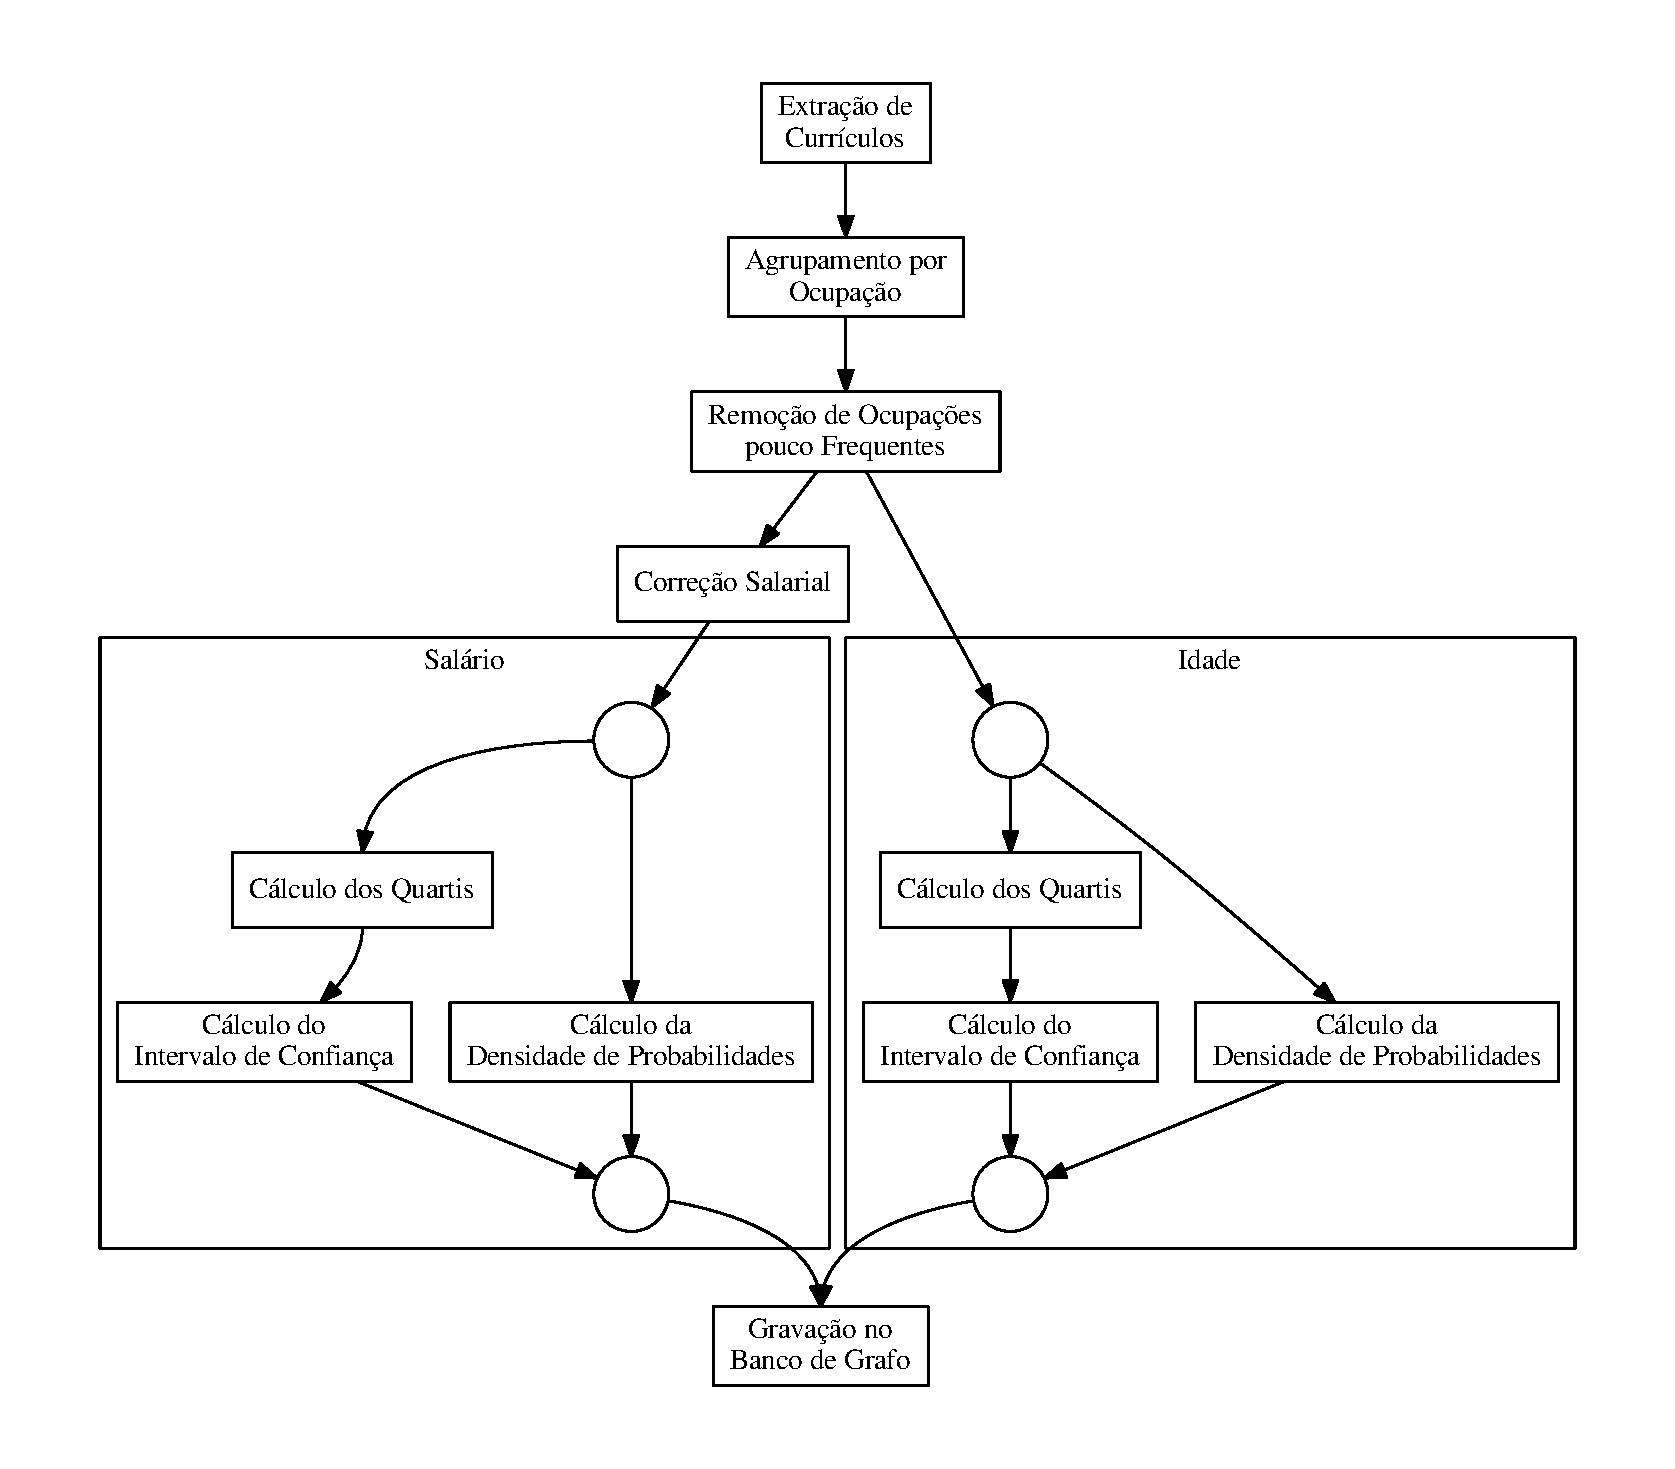
\includegraphics[scale=0.4]{pipeline2.pdf}
  \caption{Análise de Distribuição}
  \label{fig:analise-de-distribuicao}
\end{figure}

\subsubsection{Extração de Currículos}

De maneira similar ao descrito no passo~\ref{sec:extracao-experiencia}, esse processo extrai dados do banco de dados relacional e grava uma estrutura simplifica do currículo em um arquivo texto com linhas em formato JSON.

Os dados extraídos são:

\begin{itemize}
\item Nome da Última Ocupação
\item Último Salário
\item Data do Último Salário
\item Escolaridade
\item Curso da Graduação
\end{itemize}

O \textit{Nome da Última Ocupação} é o texto livre presente no campo \enquote{Cargo} da experiência profissional mais recente presente no currículo.

O \textit{Último Salário} é o valor informado pelo usuário no campo de mesmo nome. Junto a ele a \textit{Data do Último Salário} indica a qual data esse valor é referente.

A \textit{Escolaridade} é selecionada pelo usuário de uma lista pré-definida. Ela possui valores que vão de \textit{primeiro grau completo} até \textit{pós-graduação}. Para fins de análise, \textit{segundo grau incompleto} é considerado como \textit{primeiro grau completo} e \textit{graduação incompleta} é considerada \textit{segundo grau completo}.

Para os usuário com graduação ou pós-graduação como escolaridade, o campo \textit{Curso da Graduação} possui o nome do curso selecionado de uma lista de XX graduações.

\subsubsection{Normalização de Última Ocupação}

A ocupação é normalizada da mesma forma que no passo~\ref{sec:normalizacao}. O mesmo processo é aproveitado em \textit{pipelines} diferentes.

O passo de normalização permite que os dados desse \textit{pipeline} abasteçam o grafo gerado no pipeline XX.

\subsubsection{Correção Salarial}

Para que as análises sobre salários não apresentem distorções para baixo, os salários são corrigidos pelo IPCA (extraídos do site do IBGE) (ref) com base na data informada pelo usuário.

Durante esse etapa, a data do último salário é descartada pois não é mais necessária nas etapas subsequentes.

\subsubsection{Agrupamento por Ocupação}

As informações são agrupadas por ocupação. Cada ocupação passa a ser um único registro onde as outras informações estão agrupadas.

Essa transformação prepara os dados para serem convenientemente processados nas etapas posteriores.

O salário se torna uma lista ordenada, a escolaridade é transformada em um \textit{multiset} com a contagem de valores iguais e o  curso da graduação é agrupado da mesma forma.

\subsubsection{Remoção de Ocupações pouco Frequentes}

A definir\ldots

\subsubsection{Quartil Salarial}

Para cada ocupação, são calculados os três quartis do salário. Os quartis fornecem uma descrição de como a distribuição de salários se comporta. Enquanto a mediana fornece uma medida de centralidade, o intervalo interquartil descreve a dispersão dos salários.

É interessante observar que a distância entre o quartil inferior e a mediana é sempre menor do que a distância entre a mediana e o quartil superior. Isso se deve ao formato da distribuição ser inclinado à direita, o que é reconhecido com o formato da \enquote{pirâmide salarial} (ref).

Um fato importante sobre essa observação é que, para todas as ocupações, existem mais pessoas ganhando perto da base do que no topo, e por esse motivo, a maior parte dos profissionais ganha abaixo da média aritmética.

\subsubsection{Intervalo de Confiança 95\% do Salário}

Uma inspeção visual das densidades de probabilidades geradas no passo~\ref{sec:kde-salario} mostra que as probabilidades de distribuição de salário não seguem uma distribuição normal. Todas são inclinadas à direita e possuem variados graus de dispersão, para uma estimativa de intervalo de confiança seria preciso primeiro estimar a inclinação e a curtose de cada distribuição.

Também é possível notar em algumas probabilidades de densidade são multimodais ou apresentam platôs, o que inviabiliza~\todo{Meio forte isso, tem como ser mais preciso?} a aplicação das estimativas de intervalo de confiança.

A alternativa escolhida foi o uso do método de \textit{bootstrap}~\todo{Colocar Bootstrap no referencial teórico} para obter-se o intervalo de confiança 95\% do quartis salariais.

Para avaliar qual o melhor número de iterações para o \textit{bootstrap}, avaliou-se amostralmente ocupações com 1.000, 10.000 e 100.000 iterações. Para as amostras selecionadas, os resultados variavam pouco~\todo{Coletar quem foram as amostras e qual a variação encontrada} entre o número de iterações. Conservadoramente, optou-se pelo uso de 10.000 iterações para o cálculo.

\subsubsection{Densidade de Probabilidades de Salário} \label{sec:kde-salario}

Como a dispersão dos salários varia bastante entre as ocupações, as tentativas preliminares de se criar histogramas apresentavam dificuldades tanto na escolha automática da largura dos \textit{bins} quanto o ponto de partida.

Optou-se, portanto, pelo uso da densidade de probabilidades de \textit{kernel}. Esse método possui apenas um parâmetro para ajusta, a largura de banda.

O processo para a seleção da largura de banda procura pelo menor valor de largura de banda possível que não crie múltiplas modas (picos) na distribuição. Para fins de exibição para o usuário, esse método é visualmente agradável.

\subsubsection{Subgrupos Salariais} \label{sec:atributo-salarial}

\todo[inline]{Essa parte não foi feita ainda}

Os salários podem variar de acordo com uma série de fatores, experiência do profissional, porte da empresa, localização da empresa, gênero, escolaridade, entre outros.

Para descobrir quais desses fatores está correlacionada a uma diferenciação no salário, é realizado um teste de significância entre profissionais da mesma ocupação subdivididos por diversos atributos.

Os atributos que não apresentarem significância estatística acima de 0,05 são considerados não relacionados a diferenciação salarial. É possível observar que ocupações diferentes possuem atributos diferentes para a diferenciação salarial, para Copeira, por exemplo, o atributo que mais se destaca é o tamanho da empresa; já para Programador, o atributo tempo de experiência se destaca.

É tentador afirmar que esses atributos são o motivo da diferenciação, mas isso não é possível. Como um exemplo intuitivo, para Gerente de Loja não é possível saber se a presença de uma graduação causa um salário maior ou se o salário maior proporciona que o profissional consiga uma graduação.

Como o salário não se pode assumir um formato para a distribuição dos salários, os testes de significância são feitos usando XX para atributos numéricos, como o tempo de experiência e a idade, e XX para atributos categóricos como gênero.

O resultado desse passo é uma lista de atributos que possuem relevância estatística na diferenciação do salário. Esses atributos são usados em para recalcular o \textit{pipeline} de análise salarial com as amostras separadas por ocupação e pelo atributos relevantes.

O \textit{pipeline} para análise de \nameref{sec:atributo-salarial} é exibido na figura XX.

\begin{figure}[ht]
  \centering
  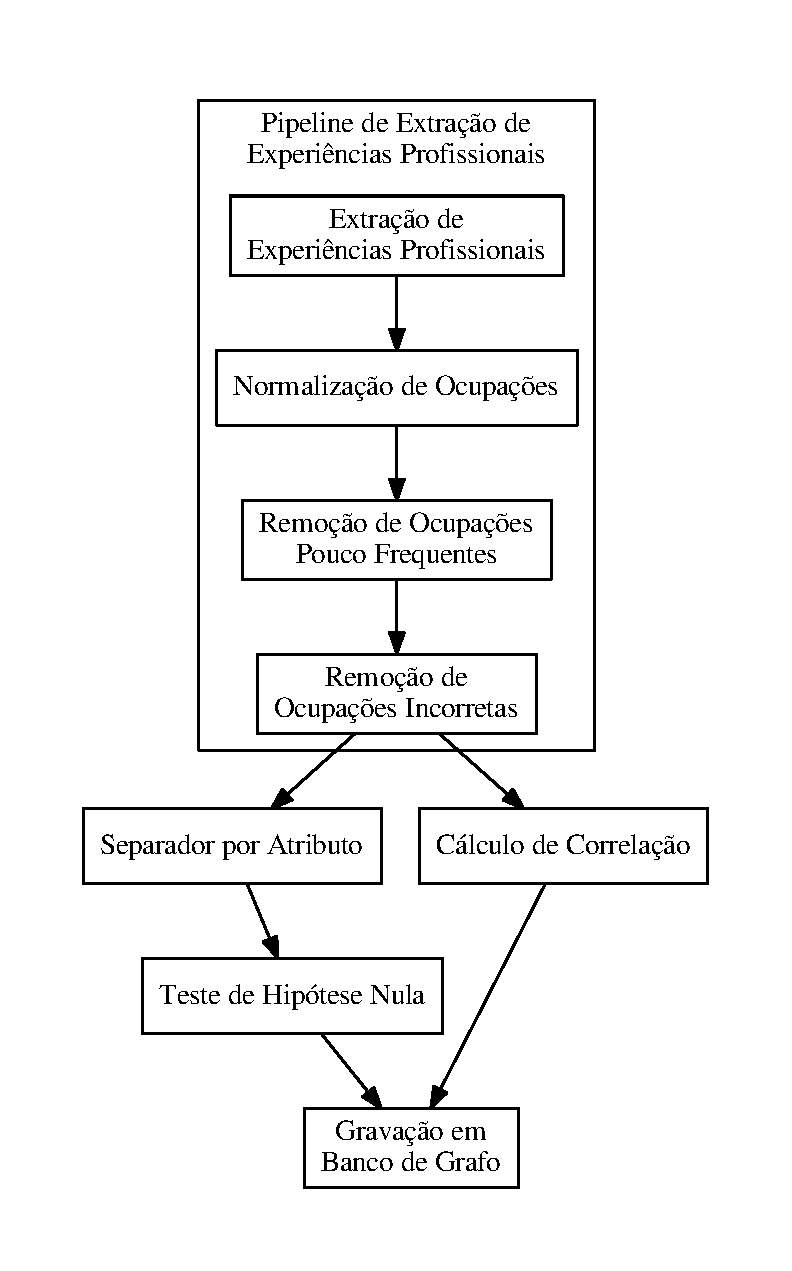
\includegraphics[scale=0.4]{pipeline3.pdf}
  \caption{análise de subgrupos salariais}
  \label{fig:atributo-salarial}
\end{figure}

\subsubsection{Densidade de Probabilidade de Tempo na Ocupação}

A definir\ldots

\subsubsection{Intervalo de Confiança do Tempo na Ocupação}

A define\ldots

\subsubsection{Gravação em Banco de Grafo}

A definir\ldots

\subsection{Análises sobre o Banco de Grafo}

\todo[inline]{Ronie: aqui é um grande ponto de indefinição, veja a seção~\ref{sec:rascunho} para algumas alternativas}

\section{Rascunho de Itens sobre a Metodologia} \label{sec:rascunho}

\todo[inline]{Toda essa seção até o cronograma ainda é um grande \textit{rascunho}. São só ideias e anotações sobre o que é possível ser feito.}

Esse pesquisa tem participação em várias etapas da projeto MCar e se estende em análises além dele.

\subsection{Montagem do a partir de uma banco relacional}

\begin{itemize}
\item Dados usados
	\begin{itemize}
	\item Experiências profissionais;
    \item Nome da ocupação;
    \item Tempo na ocupação;
	\end{itemize}
\item Preparação
	\begin{itemize}
	\item Normalização de nomes de ocupação;
	\end{itemize}
\item Montagem
	\begin{itemize}
	\item Definição de sequência de ocupações (anterior, próxima). Uso de heurística;
    \item Remoção de ocupação dupla (Diretor e Professor);
	\end{itemize}
\end{itemize}

\subsection{Análise salarial}

É possível expandir a análise para saber os componentes do salário. Alguns não estão  disponíveis, como habilidades ou empresas. Outros são mais simples, como senioridade, tempo na ocupação, escolaridade, tamanho e setor da empresa, região do país, idade e gênero. Uma análise de correlação multivariada pode identificar quais são esses componentes~\question{Ronie: Não muita certeza aqui}.

Usando a técnica de \textit{Mode Trees} é possível identificar modas na distribuição. Cada moda pode significar que existe um grupo dentro da distribuição (ref paper de mode trees).

Identificando essas modas, é possível relacioná-las com as outras variáveis descritas acima e descobrir quais causam esse agrupamento (grandes centros vs pequenas cidades, tempo de experiência, pequenas empresas vs grande empresas).

\begin{itemize}
\item Dados usados
	\begin{itemize}
	\item Experiências profissionais;
    \item Nome normalizado da ocupação;
    \item Salário;
	\end{itemize}
\item Preparação
	\begin{itemize}
    \item Remoção de outliers. Heurística: salário mínimo e salário máximo. Poda por percentil.
	\end{itemize}
\item Montagem
	\begin{itemize}
	\item KDE
    \item Bootstrap para intervalos de confiança
    \item Mode tree
    \item Identificação de picos e vales (Raízes da derivada da distribuição (analítico)? Simples comparação de vizinhança (numérico)?)
    \item Análise de correlação entre atributos e salários centrados nos picos (t-test, já que se pressupõe uma normal?)
    \item Opcionalmente, um algoritmo de predição de valor baseado nos atributos (mas não explicaria o componente do atributo em si).
	\end{itemize}
\end{itemize}

\subsection{Descrição automática do cargo}

Talvez detecção de habilidades necessárias para a ocupação?

\begin{itemize}
\item Dados usados
	\begin{itemize}
    \item Nome normalizado da ocupação
	\item Descrição do cargo na experiência profissional (o que faz)
    \item Descrição do cargo no anúncio de vaga (habilidades)
	\end{itemize}
\item Preparação
	\begin{itemize}
	\item NLP básico (tokenização, stemming)
	\end{itemize}
\item Montagem
	\begin{itemize}
	\item Anotação \textit{Part of Speech}
	\item Sumarização?
	\end{itemize}
\end{itemize}

\subsection{Predição de próximo trabalho}

\begin{itemize}
\item Dados usados
	\begin{itemize}
    \item Últimas ocupações
    \item Tempo na ocupação atual
    \item Tempo de experiência na ocupação
	\item Sexo, idade, filhos (motivadores para movimentação de carreira)
    \item Escolaridade
	\end{itemize}
\item Montagem
	\begin{itemize}
	\item Análise de similaridade de sequência
    \item ???
	\end{itemize}
\end{itemize}

\subsection{Análise de classe de ocupações}

Uma coisa que reparei enquanto montava o MCar (olhei para aqueles dados por bastante tempo) é que temos 4 tipos de trabalho que não se misturam muito. Abaixo uma descrição \enquote{no cheiro} do que observei, mas precisa de algo melhor para realmente embasar as observações abaixo.


\begin{description}
\item [Operacional] Escolaridade no 3º grau incompleto (ou menor, 2º grau é o mais comum. Contém \enquote{graduações saturadas} como Direito e Administração de Empresas. Salário é mais baixo. Grande migração entre outros cargos operacionais sem muita correlação (garçom → mascote esportivo → pedreiro → lavador de carro → manobrista → recepcionista). Parece haver uma subdivisão aqui entre operacional de escritório (recepcionista, auxiliar administrativo, \ldots) e operacional \textit{braçal} (manobrista, lavador, garçom, \ldots) Os operacionais de escritório parecem ter níveis de experiência divididos entre \enquote{Assistentes} e \enquote{Auxiliares}.
\item [Técnico] Com algumas migrações vindas do operacional. Possui 3º grau incompleto ou menor. È bastante similar ao Operacional, mas os salários são um pouco maiores e a movimentação entre cargos não correlacionados diminui. Possui níveis de experiência: \enquote{Meio Oficial} e \enquote{Oficial}. Exemplos: Soldador, Enfermeiro, Mecânico, Cozinheiro, \ldots
\item [Especialista] Com 3º completo e acima (mestrado e doutorado são mais comuns). Possui pouquíssima movimentação para ocupações não correlacionadas, exceto para área de gestão. Possui níveis de experiência \enquote{Júnior}, \enquote{Pleno} e \enquote{Sênior}. Salários são maiores. Descrição nos currículos normalmente possui habilidades e ferramentas. Exemplos: Desenvolvedores de Software, Médicos, Arquitetos, Engenheiros (todos), \ldots
\item [Gestores] Com variados graus de formação, mas os de maior salário (ou empresas maiores) possuem formação superior ou acima (especializações e MBA são mais comuns). Pouca movimentação entre cargos não correlacionados. Salários são maiores. Classificação de experiência parece ser \enquote{Supervisor}, \enquote{Coordenador}, \enquote{Gerente}, \enquote{Diretor}. Recentemente aparecem \enquote{CEO}, \enquote{CFO}, entre outros \enquote{C's}.
\end{description}

Na minha humilde opinião, esse á um trabalho que seria uma contribuição interessante para a área de RH, pois o que descrevo aí embaixo parece ser algo formalizado pela área (provavelmente), mas que poderia ganhar bases sólidas com uma análise com esse volume de dados. Um ponto particularmente interessante é que não existe uma migração muito forte de uma para o outro, ao contrário do que já vi descrito por aí: operacional → técnico → especialista → gestão. O que parece existir é uma migração muito grande dentro de cada grupo. O operacional é mais \enquote{bagunçado}, não existe um ordem, enquanto existe uma clara progressão nos outros. Também existe uma migração de Operacional para Técnico, mas quase zero de Técnico para Especialista.

\subsection{Identificação de \textit{Carreiras}}

Basicamente a clusterização já feita para separar o subgrafo da área de TI.

Existe um desafio ali que são as ocupações \enquote{hubs} que conectam tudo (vendedor, recepcionista, auxiliar administrativo).

O grupo dos cargos operacionais é muito grande e pode ser dividido.

A técnica que usei foi simples. Separar os clusters e passar novamente o algoritmo nos maiores com parametrização mais rígida (dá para automatizar esse processo). Porém sobrou o problema dos \enquote{miniclusters} com duas ou três ocupações que poderiam se juntar à outras.

Seria possível aplicar outras técnicas de agrupamento.

\section{CRONOGRAMA}

A arquitetura está concluída, bem como todo o sistema responsável pela montagem do grafo. O sistema responsável por gerar quartis, intervalos de confiança e KDEs está implementado para salário e precisa ser generalizado para outros atributos numéricos. Esse trabalho deve consumir parte de Abril e Maio.

Os componentes que testam automaticamente a detectam quais atributos estão associados a um perfil salarial diferente deve ocupar o restante de Maio e ocupar até Julho.

A parte do sistema que prevê a próxima ocupação dado um currículo inicia em Julho e se prolonga até Setembro.

Os meses finais são reservados para ajustes no sistema e na dissertação, bem como eventuais atrasos no cronograma.

O cronograma exibido na tabela~\ref{tab:cronograma}.


\begin{table}[]
\centering
\begin{tabular}{|l|l|l|l|l|l|l|l|l|l|l|l|}
\hline
Tarefa                                                                                                      & Jan                                             & Fev & Mar & Abr                      & Mai                      & Jun                      & Jul                      & Ago                      & Set                      & Out                      & Nov                      \\ \hline
\multicolumn{1}{|r|}{\begin{tabular}[c]{@{}r@{}}Sistema para\\ Montagem do Grafo\end{tabular}}              & \cellcolor[HTML]{656565}{\color[HTML]{656565} } &     &     &                          &                          &                          &                          &                          &                          &                          &                          \\ \hline
\multicolumn{1}{|r|}{\begin{tabular}[c]{@{}r@{}}Analisador de\\ Distribuições\end{tabular}}                 &                                                 &     &     & \cellcolor[HTML]{009901} & \cellcolor[HTML]{009901} & \cellcolor[HTML]{FFFFFF} &                          &                          &                          &                          &                          \\ \hline
\multicolumn{1}{|r|}{\begin{tabular}[c]{@{}r@{}}Detector de Atributo\\ Relevante para Salário\end{tabular}} &                                                 &     &     &                          & \cellcolor[HTML]{009901} & \cellcolor[HTML]{009901} & \cellcolor[HTML]{009901} &                          &                          &                          &                          \\ \hline
\multicolumn{1}{|r|}{\begin{tabular}[c]{@{}r@{}}Previsor de\\ Próxima Ocupação\end{tabular}}                &                                                 &     &     &                          &                          &                          & \cellcolor[HTML]{009901} & \cellcolor[HTML]{009901} & \cellcolor[HTML]{009901} &                          &                          \\ \hline
\multicolumn{1}{|r|}{\begin{tabular}[c]{@{}r@{}}Ajustes\\ Finais\end{tabular}}                                                                        &                                                 &     &     &                          &                          &                          &                          &                          & \cellcolor[HTML]{009901} & \cellcolor[HTML]{009901} & \cellcolor[HTML]{009901} \\ \hline
\end{tabular}
\caption{Cronograma}
\label{tab:cronograma}
\end{table}


\section{Geladeira}

Aqui fica o texto escrito e que pode ser reaproveitado em outras partes do trabalho, mas que parece que não encaixa de onde foram tirados.

\subsection{Geladeira do Referencial Teórico}

\subsubsection{Limpeza de dados}

Na limpeza dos dados aplicam-se técnicas para tratamento de dados ruidosos, remoção de inconsistências e tratamento de dados faltantes.

Por dados ruidosos, entendam-se dados que possuem variações fora do que seria considerado normal para o dado em questão~\cite{Nunes2016}. Por exemplo, pela diretriz do ensino nacional, espera-se que os alunos da 1ª série do ensino fundamental tenham entre 6 e 7 anos, um amostra que revele um aluno com 9 anos poderiam ser um \enquote{ruído}. Ruídos como esse não podem ser classificados imediatamente como inconsistências, como seria o caso de um aluno com 123 anos (além do limite humano de vida). 

Uma causa possível de ruído ou inconsistência são entradas no sistema que permitem que o usuário escreva livremente, pois o dado gerado por essa entrada é passível de erros de digitação ou pode não estar relacionado com a informação solicitada. Ruídos também podem ser causados por imprecisão na medição. No exemplo anterior, o aluno registrado com 9 anos pode realmente ter essa idade e nesse caso esse valor não é um ruído, ou pode ter na verdade 6 anos e seu registro possui um erro de digitação. Esse tipo de ruído é por vezes indistinguível dos dados legítimos, tornando sua detecção problemática. Algumas técnicas podem ser usadas para minimizar seu efeito \cite{Nunes2016}.

Para diminuir o ruído, valores numéricos podem discretizados ou então ter seu valor aproximado ao de uma função conhecida. Uma técnica de discretização seria dividir os valores em faixas (caixas ou \textit{bins}) e usá-las ao invés do valor original. Uma técnica de aproximação seria, por exemplo, sabendo-se que a distribuição do valores deveria se comportar como uma reta, usar sua fórmula para substituir o valor original pelo valor mais próximo dentro da função.
% NO PARÁGRAFO ACIMA VOCÊ FEZ UMA CONFUSÃO ENTRE SUAVIZAÇÃO, DISCRETIZAÇÃO E APROXIMAÇÃO. Ronie: Narf... vou corrigir!

Outra abordagem é o uso de técnicas resistentes a ruídos, quando disponíveis. Para a análise descritiva por exemplo, a estatística robusta é resistente a anomalias~\cite{Rousseeuw2011-nk,Hellerstein2008-zr}.
% OUTRA ABORDAGEM PARA QUE? Ronie: A intenção original era descrever a abordagem "padrão" e a que eu usei.
% E ESSA HISTÓRIA DE ESTATÍSTICA ROBUSTA? NÃO PRECISAMOS DELA. Ronie: Pois é... mas é justamente por ter problemas com anomalias que recorri a ela. Tb teve uma questão que é mais fácil explicar ao vivo, mas ela é ilustrada pela afirmação: "Mais da metade das pessoas ganha menos do que a média salarial" :)
% NORMALMENTE NOS REFERIMOS A "SENSIBILIDADE A RUÍDO" E NÃO "RESISTÊNCIA A RUÍDO". Ronie: Seria correto dizer "menos sensível a ruídos"?

Para dados textuais, uma variedade de ruídos que deve ser considerada são os erros de digitação. O tratamento mais comum para esse tipo de erro é o uso de um dicionário eletrônico e algoritmos como o \enquote{edit distance} descrito por \citeonline{Norvig2007-cz}. Ele é especialmente útil quando o texto possui jargões e um dicionário pode ser construído a partir dos dados.
% SE A GENTE NÃO DEIXAR CLARO ONDE PODE HAVER RUÍDO NOS NOSSOS GRAFOS DE CARREIRA, VAI FICAR DIFÍCIL ESCREVER UM TEXTO FLUIDO. Ronie: A montagem básica tem ruído no texto, depois aparece no tempo de permanência, salário, palavras chaves e bom... as outras informações "extras".

Dados inconsistentes, por sua vez, são dados que estão fora dos limites aceitáveis para a informação sendo trabalhada, como o aluno de 123 anos no exemplo anterior. Também são chamados inconsistentes os dados que não são aplicáveis ao domínio do atributo, como o texto "NÃO" em uma informação relacionada a idade, ou quando a mesma informação é registrada com diferentes valores em diferentes locais na base de dados.~\cite{Nunes2016} Algumas inconsistências são facilmente detectáveis, enquanto outras precisam de intervenção manual. A participação de especialistas de negócio em alguns casos é essencial. Dependendo da inconsistência, o dado pode ser tratado de maneira similar ao dado com ruído, ou então ele deve ser removido do conjunto de dados.

Finalmente, dados faltantes estão relacionados a simples omissão do dado, intencional ou não. O tratamento desse tipo de dado vai de estratégias simples, como ignorar o objeto que possui o dado faltante até estratégias complexas como criar um modelo preditivo para imputar o valor faltante.
% PADRONIZE A NOMENCLATURA. SE FOR USAR DADO FALTANTE, ENTÃO USE APENAS FALTANTE, MAS SE FOR PARA AUSENTE, AUSENTE SERÁ! PARTICULARMENTE PREFIRO VALORES AUSENTES. NOTE QUE UM VALOR AUSENTE É DIFERENTE DE UM DADO AUSENTE, POIS A PALAVRA DADO SE REFERE A OBJETO, ENQUANTO VALOR ESTÁ ASSOCIADO A UM CAMPO QUALQUER DA BASE (TABELA). DETECTAR UM DADO AUSENTE REQUER CONHECIMENTO ESPECIALISTA, POR EXEMPLO, PARA EU SABER SE UM ALUNO ESTÁ AUSENTE AD LISTA DE CHAMADA EU PRECISO SABER QUE ESSE ALUNO DEVERIA ESTAR ALI. POR OUTRO LADO, SE O ALUNO ESTIVER NA LISTA E FALTAR UMA NOTA PARA ELE, EU AUTOMATICAMENTE VEJO. PARECE SUTIL A DIFERENÇA, MAS NÃO É. Ronie: Boa... valor ausente será :)

As técnicas mencionadas acima são aplicadas em maior ou menor grau nesse trabalho, entretanto, algumas são especificamente importantes pois as etapas seguintes dependem da sua aplicação. Abaixo descrevemos essas técnicas.

\subsubsection*{Normalização de Termos}
% POR QUE VOCÊ VAI FALAR DE NORMALIZAÇÃO DE TERMOS AQUI? Ronie: Boa! Vai pra dentro de Mineração de Texto.
A normalização de termos é uma técnica usada na área da Recuperação de Informação para que os resultados sejam mais próximos da intenção do usuário~\cite{Manning2008-fw}. Ela é aplicada na etapa de preparação dos dados e vai além de lidar com dados com ruído, embora essa seja uma de suas funções.

No texto escrito é comum que palavras tenham grafias diferentes mas mesmo significado. Abreviações como \enquote{aux.} significando \enquote{auxiliar}; \enquote{ZL}, \enquote{Z.L.}, \enquote{Zona Leste} ou \enquote{zona leste}; ou simplesmente singular e plural como \enquote{porta} e \enquote{portas}. Também por erro, preferência do usuário ou dificuldades na entrada de dados, palavras são escritas sem acentuação: \enquote{Sao Paulo} ao invés de \enquote{São Paulo}.

Uma das técnicas mais comuns para lidar com esse problema consiste em eleger um termo \enquote{canônico} para representar todas as variantes relacionadas e estabelecer um dicionário de equivalência~\cite{Manning2008-fw}. É importante observar que um termo canônico não é o mesmo que \textit{lema}, pois esse último é um termo presente no dicionário que contém o significado base da palavra, enquanto que o termo canônico precisa apenas ser uma representação para a qual termos equivalentes possam ser reduzidos. Por exemplo, o termo canônico para "São Paulo" pode ser "SP", mas "SP" não é um lema válido.

Algumas normalizações são processáveis com uma heurística simples, como remover a pontuação em abreviações como \enquote{Z.L.} e \enquote{ZL}, dispensando a necessidade de uma extensa enumeração de todas as variações possíveis. Outras, no entanto, só são possíveis com conhecimento do negócio ou com algoritmos mais sofisticados, como a equivalência entre os termos \enquote{carro} e \enquote{automóvel}.

Outra equivalência simples é a remoção de acentuação (diacríticos) e a transformação dos termos para minúscula (\textit{case-folding}). Esses são dois processos comuns para a normalização de termos~\cite{Manning2008-fw}. Contudo, é importante notar que algumas palavras na língua portuguesa diferem apenas pelo acento, chamadas \enquote{homógrafos imperfeitos}, como em \enquote{cítara} (instrumento) e \enquote{citara} (verbo mencionar), \enquote{maçã} (fruta) e \enquote{maça} (arma medieval), \enquote{saia} (vestimenta) e \enquote{saía} (verbo sair). Esses casos são pouco comuns e, via de regra, os erros causados por acentos ausentes ou mal colocados causam mais distorção do que a colisão de significado entre homógrafos imperfeitos.

Outras equivalências envolvem trabalho manual ou aprendizado de máquina como as observadas em trabalhos como \citeonline{Jijkoun2008-ie} ou \citeonline{Jacob2014-cf} que lidam com normalização de entidades.

Também é possível a aplicação de dicionários de sinônimos, porém essa abordagem é limitada segundo o tipo de texto sendo processado. No caso de textos específicos de negócio, o jargão da área se sobrepõe ao sinônimo comum. Por exemplo, no setor de logística terrestre, o \enquote{caminhão} é chamado \enquote{carro} e um \enquote{automóvel} é por vezes chamado de \enquote{viatura}, a parte do caminhão composta apenas pela cabine, motor e rodas de tração é chamada \enquote{cavalo} (uma simplificação de \enquote{cavalo mecânico}).

O uso de um dicionário genérico de sinônimos em situações como a descrita acima pode causar distorção nas análises. Nesses casos, a elaboração de um dicionário específico de negócio é uma solução limitada, mas possível. Se o domínio de negócio possuir uma grande concentração de registros em poucos termos, um dicionário de tamanho reduzido pode tratar uma grande parte dos dados.

Por exemplo, os termos \enquote{auxiliar} e \enquote{assistente} estão presentes em uma grande parte das ocupações mapeadas no presente trabalho. Um pequeno dicionário com suas versões abreviadas \enquote{aux}, \enquote{assist} e \enquote{ass} reduz o número de ocupações com esses termos de 35\% para 21\%, eliminando a redundância.

Continuando o exemplo, apesar dos dois termos parecerem equivalentes, eles possuem significados diferentes. Quando o assunto é ocupação, o \enquote{assistente} é considerado uma ocupação de nível superior ao \enquote{auxiliar}. Um dicionário que os transformasse em termos equivalentes perderia um significado importante para o trabalho.

\subsubsection*{Extração do Radical de Termos}
% ATÉ ESTE MOMENTO NÃO ESTÁ CLARO PARA MIM A MOTIVAÇÃO EM APRESENTAR MUITOS DOS CONCEITOS AQUI. ISSO DEVE FICAR CLARO QUANDO EU ENTENDER MAIS PRECISAMENTE QUAIS ANÁLISES SERÃO FEITAS NOS GRAFOS. Ronie: até aqui foram só coisas que usei para a montagem do grafo, na verdade :( 
A extração do radical dos termos (\textit{stemming}) também é uma técnica bastante utilizada, é difícil encontrar um livro sobre mineração de textos que não a mencione. Ligeiramente diferente da normalização, o objetivo da extração do radical é preservar o sentido geral da palavra.

Um dos melhores algoritmos de \textit{stemming} para a língua portuguesa é uma adaptação do algoritmo de Porter chamado \textit{RSLP Stemmer}~\cite{Flores2010-gk}. A algoritmo de Porter é basicamente uma lista de substituições aplicadas sequencialmente, removendo sufixos, mas não prefixos.

O RSLP está disponível como \textit{stemmer} padrão no pacote de processamento de linguagem natural do Python (NLTK). Ele adapta o Porter com uma lista de exceções para evitar que o algoritmo remova sufixos indevidamente, evitando que ele unifique palavras como \enquote{cama} e \enquote{caminho} no radical \enquote{cam}~\cite{Orengo2001-yw}.

Entretanto, mesmo o RSLP ainda não é perfeito, casos como \enquote{solda\textbf{dor}} e \enquote{solda\textbf{do}} são ambos reduzidos para \enquote{sold}. Em um texto genérico os benefícios do \textit{stemming} superam o problema causado por erros como esse~\cite{Hollink2004-hh}. Entretanto, para o presente trabalho, que visa agrupar ocupações profissionais, esse tipo de erro unifica profissionais bastante diferentes. Outras estratégias foram aplicadas no intuito de aumentar a confiabilidade dos resultados.\footnote{Ronie: Talvez esse parágrafo devesse ser colocado mais para frente, quando mencionar o trabalho em si}

\def\refname{REFERÊNCIAS BIBLIOGRÁFICAS}
\bibliography{biblproj}
\addcontentsline{toc}{section}{REFERÊNCIAS BIBLIOGRÁFICAS}
\bibliographystyle{abnt-alf}

\end{document}
